%
%
%
%
%

%
%

%
%
%
\section{Introduction}
%

%
%
%
%
%
%
%
%
%

Beta-band oscillatory activity and exaggerated bursting in the STN-GPe network
are key features of parkinsonian pathophysiology that are correlated with its
akinetic-bradykinetic motor symptoms \cite{sharott_dopamine_2005,mallet_disrupted_2008,kuhn_high-frequency_2008,sanders_parkinsonism-related_2013,sharott_activity_2014}. Moreover, improvements in those symptoms correlate
with their suppression by DBS. Hence, capturing these features is essential
for computational models whose purpose it is to optimize DBS stimulation protocols.
The biophysically detailed network model of the STN-GPe loop presented in
Chapter~\ref{ch3:detailed-model} exhibited spontaneous beta-band synchronization and
resonance behavior in Parkinsonian conditions, and synchronization in the network
occurred together with strong burst firing in STN neurons. However, because of
the biophysical detail captured by the model, it consists of a large number of
state variables and high computational complexity.
This leads to long simulation times that make the model impractical
for the efficient exploration of DBS parameter settings, where simulation of large
numbers of neurons at very small timescales is required.
%
%
%
%
%
%
%
Moreover computational complexity limits the ability to scale up
the size of the network to realistic numbers of neurons, equaling approximately
13,000 cells in the rat subthalamic nucleus (STN) and 30,000 in the external
globus pallidus (GPe), unilaterally \cite{oorschot_absolute_1999,abdi_prototypic_2015}.

At the same time, the high level of biophysical detail captured by the model
confers it with several key advantages. First, the neuron models used
can reproduce spiking features that are mediated by the interaction between
dendritic ion channels and synaptic currents. Indeed, bursting in STN neurons
is a phenomenon mediated by the generation of  voltage plateaus originating
from $Ca^{2+}$ influx in distal dendrites \cite{gillies_membrane_2005}.
In addition to network topology and synaptic strengths, dendritic processing
of synaptic inputs also influences the synchronization properties of neurons,
both by passive propagation and by the engagement of active ion channels
\cite{schultheiss_phase_2010,goldberg_response_2007}.
%
Another major advantage of detailed multi-compartment models is that the effects of
extracellular electrical stimulation can be modeled using spatially varying
extracellular potentials. This captures its distributed interaction with the
membrane rather than assuming a single equivalent source modifying the neuron's output,
often located at the soma.
%


To preserve the advantages of the biophysically detailed model it is
desirable to have an intermediate level of description that retains
its straightforward relation to the underlying biophysiology of the system
while reducing the computational complexity of the model to achieve computational
efficiency. One way to address this problem, is the use of methods for
the systematic reduction of detailed morphological neuron models into
equivalent cable models. Such methods were explored
early in the development of neuronal cable models, starting with the
`3/2 rule' for collapsing passive branching structures into
analytically equivalent cylinders \cite{rall_branching_1959,rall1964theoretical}.
This rule states that neurites originating at a branch point can be replaced
by an equivalent cylinder that preserves passive outward voltage attenuation
if the branch point obeys the 3/2 power rule. In short, the sum of the 3/2 power
of child branch diameters must equal the 3/2 power of the parent branch diameter,
biophysical properties must be uniform, and the child branches must terminate
at the same electrotonic distance from the branch point.
These limitations were relaxed in subsequent reduction methods, producing
equivalent cables for passive dendrites with arbitrary geometries, in terms
of outward voltage attenuation  \cite{clements1989cable,stratford1989modelling,douglas1992exploring,ohme1998equivalent,fleshman1988electrotonic,evans2000analysis}.
%
However, because local input impedances are altered by those methods,
voltage transients in response to dendritic current sources are not
preserved. This means that the local effects and inward propagation of
transients evoked by active ion channels or synaptic currents are not preserved.
To address the case of nonlinear ionic and synaptic conductances in the dendrites,
heuristic methods were developed that preserve certain key electrical properties
but these often require additional fitting or manual fine tuning steps
\cite{traub_model_1991,bush_reduced_1993,pinsky_intrinsic_1994,davison_reduced_2000,marasco_fast_2012}.

%
%
%
%
Despite their ability to substantially reduce the computational complexity of
branching neuron models, morphology reduction methods are limited in their ability
to accurately preserve the full spectrum of responses of detailed models \cite{hendrickson_capabilities_2011,elbasiouny_development_2014}.
Most importantly, all morphology reduction methods suffer from the input impedance problem
\cite{deschutter2000computational} where the local input impedance seen at points on the
dendrites is different from that in the original model. As a result, dendritic current
sources such as synapses will generally not produce identical voltage transients
and, therefore, their coupling to voltage-sensitive ionic conductances is altered.
Moreover, after collapsing dendritic branches, synapses that were originally spatially and
electrically isolated are mapped to the same location, reducing voltage
compartmentalization and introducing mutual shunting effects.
As a result of these limitations, neuronal responses that depend strongly on
dendritic input impedance and activation of dendritic active channels are
generally not accurately reproduced when the reduction eliminates a high
degree of branching \cite{hendrickson_capabilities_2011,elbasiouny_development_2014}.
%
Nevertheless, intermediate levels of reduction that preserve a certain
degree of branching can be used to reproduce key features of the neuron's responses
\cite{hendrickson_capabilities_2011,elbasiouny_development_2014}.
If these features are sufficient to preserve key properties of
neuronal network behavior, morphology reduction would be a suitable strategy
to study the network effects of physiological and electrical interventions such
as deep brain stimulation (DBS). The capabilities of reduced morphology models
to reproduce single cell responses of their more detailed counterparts
were investigated systematically in \cite{hendrickson_capabilities_2011} for GPe neurons and in \cite{elbasiouny_development_2014} for motor neurons.
However, their ability to reproduce neuronal network activity and network
synchronization properties has not yet been investigated. %

%
From the perspective of network synchronization,
one way to quantify how well the features of a neuron's response properties
are captured by an equivalent model are phase response curves (PRC).
%
%
%
%
%
%
In general, PRC quantify the phase perturbation of an oscillating system
in response to an input arriving at a specific phase of its ongoing oscillation.
In neurons, therefore, PRC give the phase advance or delay of the following spike
as a function of the phase at which an input arrives during the inter-spike interval (ISI).
An important theoretical result is that the shape of the PRC predicts the
tendency of neurons to synchronize to oscillatory inputs, and can also predict
synchronization patterns arising in mutually connected populations of
oscillating neurons, depending on their connection types \cite{hansel_synchrony_1995,ermentrout_type_1996,goldberg_response_2007,achuthan_phase-resetting_2009,bogaard_interaction_2009,abouzeid_type-ii_2009}.
%
%
%
%
%
%
%
%
Moreover the shape of the PRC is determined by both passive filtering
properties of dendrites and nonlinearities introduced by active conductances
\cite{goldberg_response_2007,gutkin_phase-response_2005,crook_dendritic_1998},
which are present in GPe and STN neuron dendrites. It may, therefore, be expected
that PRC provide a suitable way to compare the characteristics of candidate
model neurons when the aim is to investigate network synchronization properties.
%
%
%
%
%
%
%


%
Therefore the aim of this study was to reduce the biophysically detailed network
model of the STN-GPe loop presented in Chapter~\ref{ch3:detailed-model} to
a more tractable number of compartments while maintaining key features
of network activity and its frequency response. To achieve this, a morphology
reduction algorithm was applied that reduced the detailed multi-compartmental
neuron models to equivalent cable models consisting of fewer compartments.
To gauge whether the essential input-output characteristics of the model neurons
were captured before simulating the complete network, two methods were used.
First, responses of model neurons to current clamp protocols designed to elicit
stereotypical responses were compared to ascertain that crucial features such as bursting
and spontaneous oscillations were conserved.
%
%
Second, phase response curves of the model neurons were compared
to measure how model neurons synchronized to their synaptic inputs.
%
%
Finally, the behaviour of the reduced network model was compared with that
of the full model presented in Chapter~\ref{ch3:detailed-model} to investigate
whether synchronization properties, neuronal activity patterns, and the network
response to cortical oscillatory inputs were preserved.

%
%
%

%
%
%
%
%
%
%
%

%
%
%
%
%
%
%

%
%
%
%
%
%
%
%
%
%
%
%

%
%
%
%
%
%
%
%
%
%
%
%

%
%
%
\section{Methods}
%
%

%
%
%

\subsection{Morphology reductions}

%
%
%
%
%
%
%
%
%


An algorithm for reducing the number of compartments of conductance-based
neuronal cable models by constructing equivalent cables was developed.
The algorithm for clustering compartments and calculating properties
of the equivalent cables was adapted from the algorithms described in
\cite{bush_reduced_1993,marasco_fast_2012,douglas1992exploring}.
%
Dendritic regions were first defined in the STN and GPe neuron models based
on their distance from the soma \cite{douglas1992exploring}. Starting at the trunk section of each
primary dendrite $D$ attached to the soma, compartments located at distance $x$ from the
soma, where $ n \Delta L \leq x \le (n+1) \Delta L $ were assigned to cluster $D_n$.
The spacing $\Delta L$ was set to 50 micron in STN neurons and 1 micron in GPe neurons.
In GPe neurons, the spacing was much smaller because dimensions of the original
\cite{gunay_channel_2008} GPe neuron model were normalized to 1 micron resulting
in very short lengths of dendritic branches (see discussion).
%

%
%
%
%
%
%
%
%
%
%
%
%
%
%
%
%
%
%
%

Next, each cluster of compartments $D_n$ was represented by an equivalent cable,
with dimensions and biophysical properties determined using the equations described
in \cite{marasco_fast_2012}. The equations are based on those of \cite{bush_reduced_1993}
and are designed to yield equivalent cables with axial resistance per unit length equaling
that of the collapses branches connected in parallel. In each cluster, sequentially
connected compartments were first combined yielding cables with equivalent
length $L_{seq}$ and diameter $d_{seq}$:

\begin{align}
    L_{seq} &= \sum_i^N L_i \\
    d_{seq} &= \sqrt{\frac{ 4 L_{seq} R_a }{ \pi \sum_i^N R_i }}
\end{align}

where $L_i$ is the length of sequential compartment i, $Ra$ is the axial
resistivity in $\Omega$cm (typically assumed constant in a neuron, as in the
models used here), and $R_i$ is the absolute axial resistance in $\Omega$
defined as $R_i = \frac{4 R_a L_i}{\pi d^2}$. This
ensures that the axial resistance $R_i$ is conserved in the equivalent cable.
Then, the resulting parallel cables in the cluster were combined using equivalent length and diameter

\begin{align}
    L_{br} &= \frac{ \sum_i^N S_i L_i }{ \sum_i^N S_i } \\
    d_{br} &= \sqrt{ \sum_i^N d_i^2 }
\end{align}

resulting in an equivalent axial resistance equal to a parallel circuit of merged
axial resistances.
Finally, all membrane conductances $\overline{g}_k$ and capacitances $c_{m,k}$
in the original cable were scaled by the ratio of original to equivalent
surface area $c_k$ of cluster $k$:

\begin{align}
    c_k                     &= \frac{\sum_i^N S_i}{S^{eq}_k} \\
    \overline{g}^{eq}_k     &= \overline{g}_k c_k \\
    c_{m,k}^{eq}                &= c_{m,k} c_k
\end{align}

where $S_i$ is the surface area of compartment $i$ belonging to cluster $k$, $S^{eq}_k$ is
the surface of the equivalent cable for cluster $k$, and $ \overline{g}^{eq}_k $
and $c^{eq}_{m,k}$ are the equivalent membrane conductances and capacitance in cluster $k$.

Using these parameter choices for the reduction algorithm, the number of compartments
in the STN cell model was reduced from 189 to 30. In the GPe cell model the number of
compartments was reduced from 141 to 19. As a result, the total number of compartments
in the STN-GPe network model was reduced from 23550 to 3400 representing a reduction
by 85.5\%.

\subsection{Network model}

The structure and connectivity of the STN-GPe network model was as described in
%
Chapter~\ref{ch3:detailed-model}, except for the neuron models used to
represent STN and GPe cells. For the cell models, the reduced STN and GPe
cell models were substituted for the original, detailed morphology models.
Synapse locations were determined randomly according to the same
spatial distributions as in the original network model.
%
%
%
While all spike trains emitted by noisy spike generators
were identical, the membrane noise current in each neuron was not necessarily the same
as random number generators were initialized differently in each simulation.
%
%
The cell populations and their connectivity patterns were unchanged:
the network consisted of four populations of neurons (Fig.~\ref{fig:network_diagram}):
the STN and GPe neurons and their cortical (CTX) and striatal (MSN) inputs, modeled as spike generators.
The STN and GPe populations consisted of 50 and 100 cells, respectively,
with 10\% of cells in each of those populations modeled as Poisson spike generators
as an additional source of random noise in the network. The cortical and
striatal populations consisted of 1,000 and 2,000 cells, respectively,
modeled as spike generators.

%
%
%
%
%
Connection patterns between the populations were determined stochastically by
randomly selecting a fixed number of afferents from the pre-synaptic population
for each post-synaptic cell. The same connectivity patterns were used as in the
detailed network model.


\subsection{Simulation details}

The network and cell models were simulated in the NEURON simulation environment \cite{hines_neuron_1997}
and implemented in Python. The default fixed time step integrator with a
time step of 0.025 ms was used for all simulations.
Network simulations were run on the UCD Sonic cluster using 12 parallel processes per simulation
on a single computing node consisting of two Intel Intel Xeon Gold 6152 CPUs (22 cores per CPU)
and 384 GB memory. The reduced network model was simulated for 7 seconds in 110 seconds CPU time, which
represents a reduction of 79\% over the detailed model which took 521 seconds of total
CPU time to simulate.

\subsection{Electrotonic properties}
%
Input and transfer impedances were calculated using the NEURON impedance
tools that use the analytical solutions for linear cable models described
in~\cite{butz_transient_1974,koch_simple_1985}. For the calculation of input
and transfer impedances, all nonlinear ionic conductances
were set to their steady state values for a transmembrane potential of -65 mV.
%

\subsection{Phase response curves}
%

%
The phase response curve describes the phase advance (positive)
or delay (negative) of an oscillating system in response to an input as a function
of the phase at which it arrives \cite{gutkin_phase-response_2005}.
In neurons, therefore, it describes the advance or delay of the next spike time
as a function of the stimulus time in the inter-spike interval (ISI).
%
PRCs were measured using synaptic inputs in STN and GPe neuron models during
positive current injection, while cells were firing at 20 Hz.
%
In the STN neuron models, glutamergic synaptic inputs were located distally and
proximally to the soma conforming to experimentally reported synapse distributions \cite{bevan_glutamate-enriched_1995,mathai_reduced_2015,pan_neuronal_2016}. In the GPe
models, a glutamergic synapse was placed distally to the soma \cite{shink_differential_1995}.
In both models, an inhibitory GABAergic synapse was placed in the perisomatic region,
proximal to the soma \cite{smith_topographical_1990,chan_hcn2_2004,sadek_single-cell_2007}.
Synaptic inputs were modeled as bi-exponential synapses with reversal potentials of
0 mV and -80 mV to model glutamergic and GABAergic synapses respectively. Rise and decay
time constants were 1 ms and 3 ms for glutamergic synapses, and 1 ms and 12 ms for
GABAergic synapses, respectively.
%
A single synaptic stimulus was administered in each ISI, its phase $\phi$ was recorded,
and the phase advance or delay $\Delta \phi$ of the following spike was recorded.
This resulted in a sample $ (\phi, \Delta \phi)$ where:

%
%
%
\begin{align}
    \phi &= (t_s - t_{spk,i-1}) / T_{mean} \\
    \Delta \phi &= 1 - (T / T_{mean})
\label{eq:prc-samples}
\end{align}

with $t_s$ equal to the arrival time of the spike at the stimulated synapse,
$t_{spk,i-1}$ the last spike time of the neuron, $T$ the inter-spike interval measured
between $t_{spk,i-1}$ and the next spike time $t_{spk,i}$ after the synaptic stimulus,
and $T_{mean}$ the mean inter-spike-interval over the stimulation/measurement period.

Sampling the PRC during positive current injection rather than during spontaneous
firing enabled a more rapid sampling of the PRC than if cells were allowed to spike
at their lower resting rates, and brought the excitation level and firing rate closer
to the situation in the network.
%
The ISI was sampled with a sampling interval of 2 ms, and 10 measurements for each time
point in the ISI were obtained during a single simulation run.
This resulted in a total simulation time of approximately 12500 ms
(50 ms / 2 ms $\times$ 10 repetitions $\times$ 50 ms) per PRC. The stimulus times in
successive ISIs were randomized to obtain 10 measurements per
time point within the ISI while introducing variability in the neuron's state variables.
The reference ISI used to calculate stimulus phases was equal to the mean ISI
during measurement of a PRC.
%
%



%
%
%
\section{Results}

%
%
%
%

%
%
%
%
%
%
%

%
%
%
\subsection{Electrical characterization of neuron models}
%

%
%
%
%
%

%
%
%
%
%
%
%
%

The model reduction yielded reduced morphologies consisting of three equivalent
cylinders representing the dendrites in both the STN and GPe neuron models
(Fig.~\ref{fig:stn-full-vs-red_Zin-Ztr}, \ref{fig:gpe-full-vs-red_Zin-Ztr}).
The input impedance seen at the soma was maintained using this method,
with an accuracy of $\leq$ 0.1 \% (Fig.~\ref{fig:stn-full-vs-red_Zin-Ztr}.A, \ref{fig:gpe-full-vs-red_Zin-Ztr}.A).
However, the local input impedance seen at points along the dendrites deviated from the
detailed models with increasing distance
from the soma because of the higher neurite diameter and membrane conductances introduced by
the equivalent cable method. Transfer impedances between different areas of the cell and the soma,
characterizing the impact of local current sources on the somatic membrane voltage, were well
maintained in the reduced models (Fig.~\ref{fig:stn-full-vs-red_Zin-Ztr}.B, \ref{fig:gpe-full-vs-red_Zin-Ztr}.B).

\begin{figure}[ht]
\centering
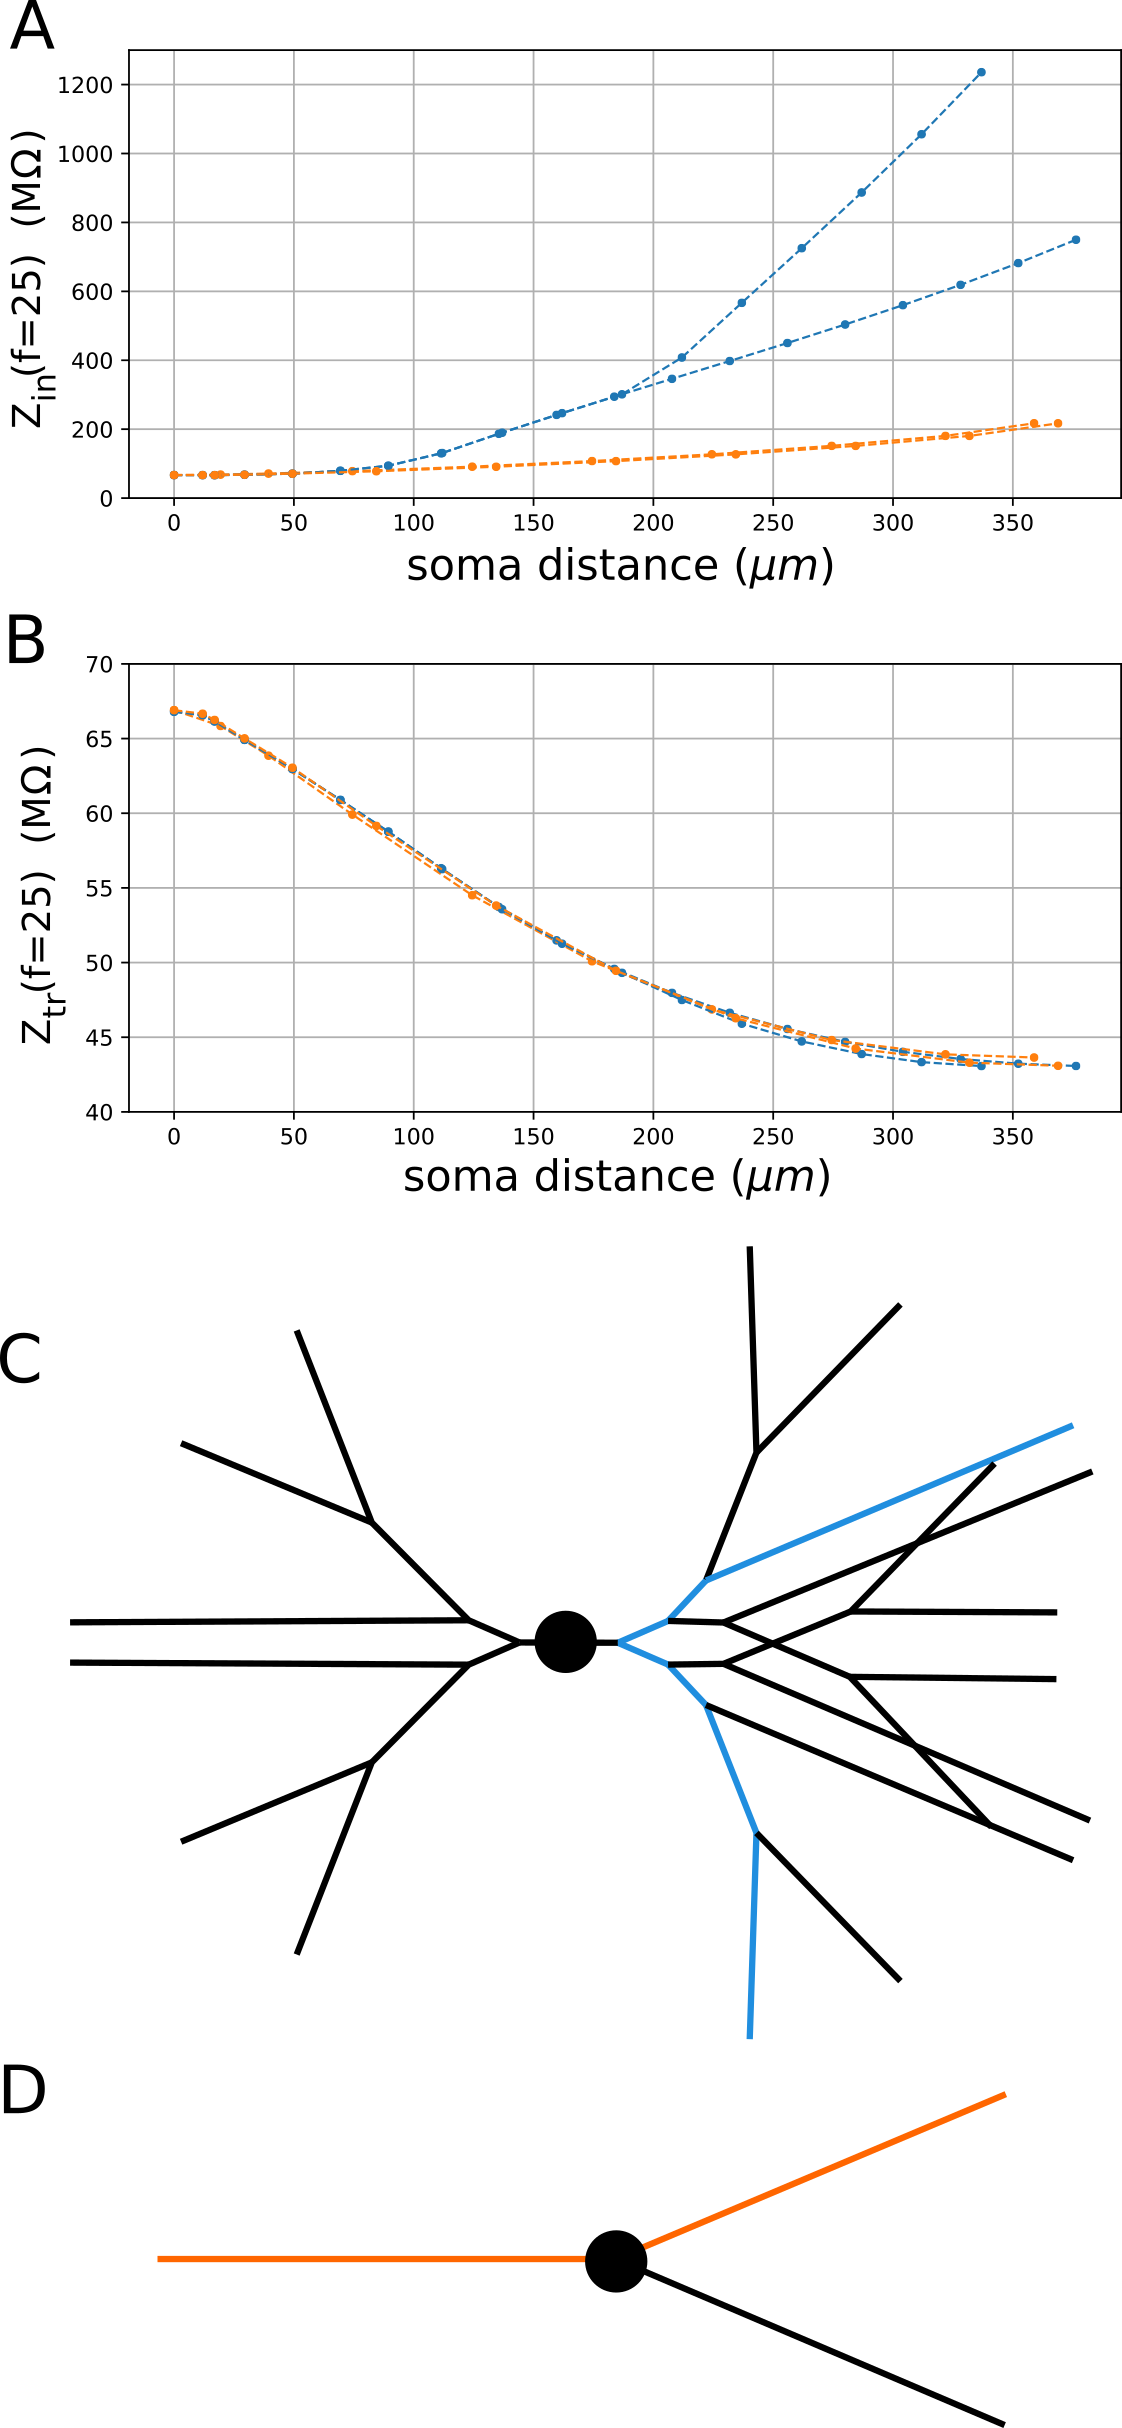
\includegraphics[height=\dimexpr \textheight - 9\baselineskip\relax]{ch_reduced_model/figs/fig_stn-full-vs-red_Zin-Ztr.png}
\caption{
\textbf{Morphological and electrical characteristics of detailed and reduced STN neuron models.}
\textbf{A}: Local input impedance seen at different points in the dendritic tree, as a function
of distance from the soma.
\textbf{B}: Local transfer impedance to the soma for current sources located at different points
in the dendritic tree.
\textbf{C}: Schematic diagram of the detailed STN neuron morphology. Paths along dendrites where
input and transfer impedances were measured are highlighted in blue.
\textbf{D}: Schematic diagram of the reduced STN neuron morphology. Dendrites are represented by
three equivalent cylinders. Paths where input and transfer impedances were measured are highlighted
in orange.
}
\label{fig:stn-full-vs-red_Zin-Ztr}
\end{figure}


\begin{figure}[ht]
\centering
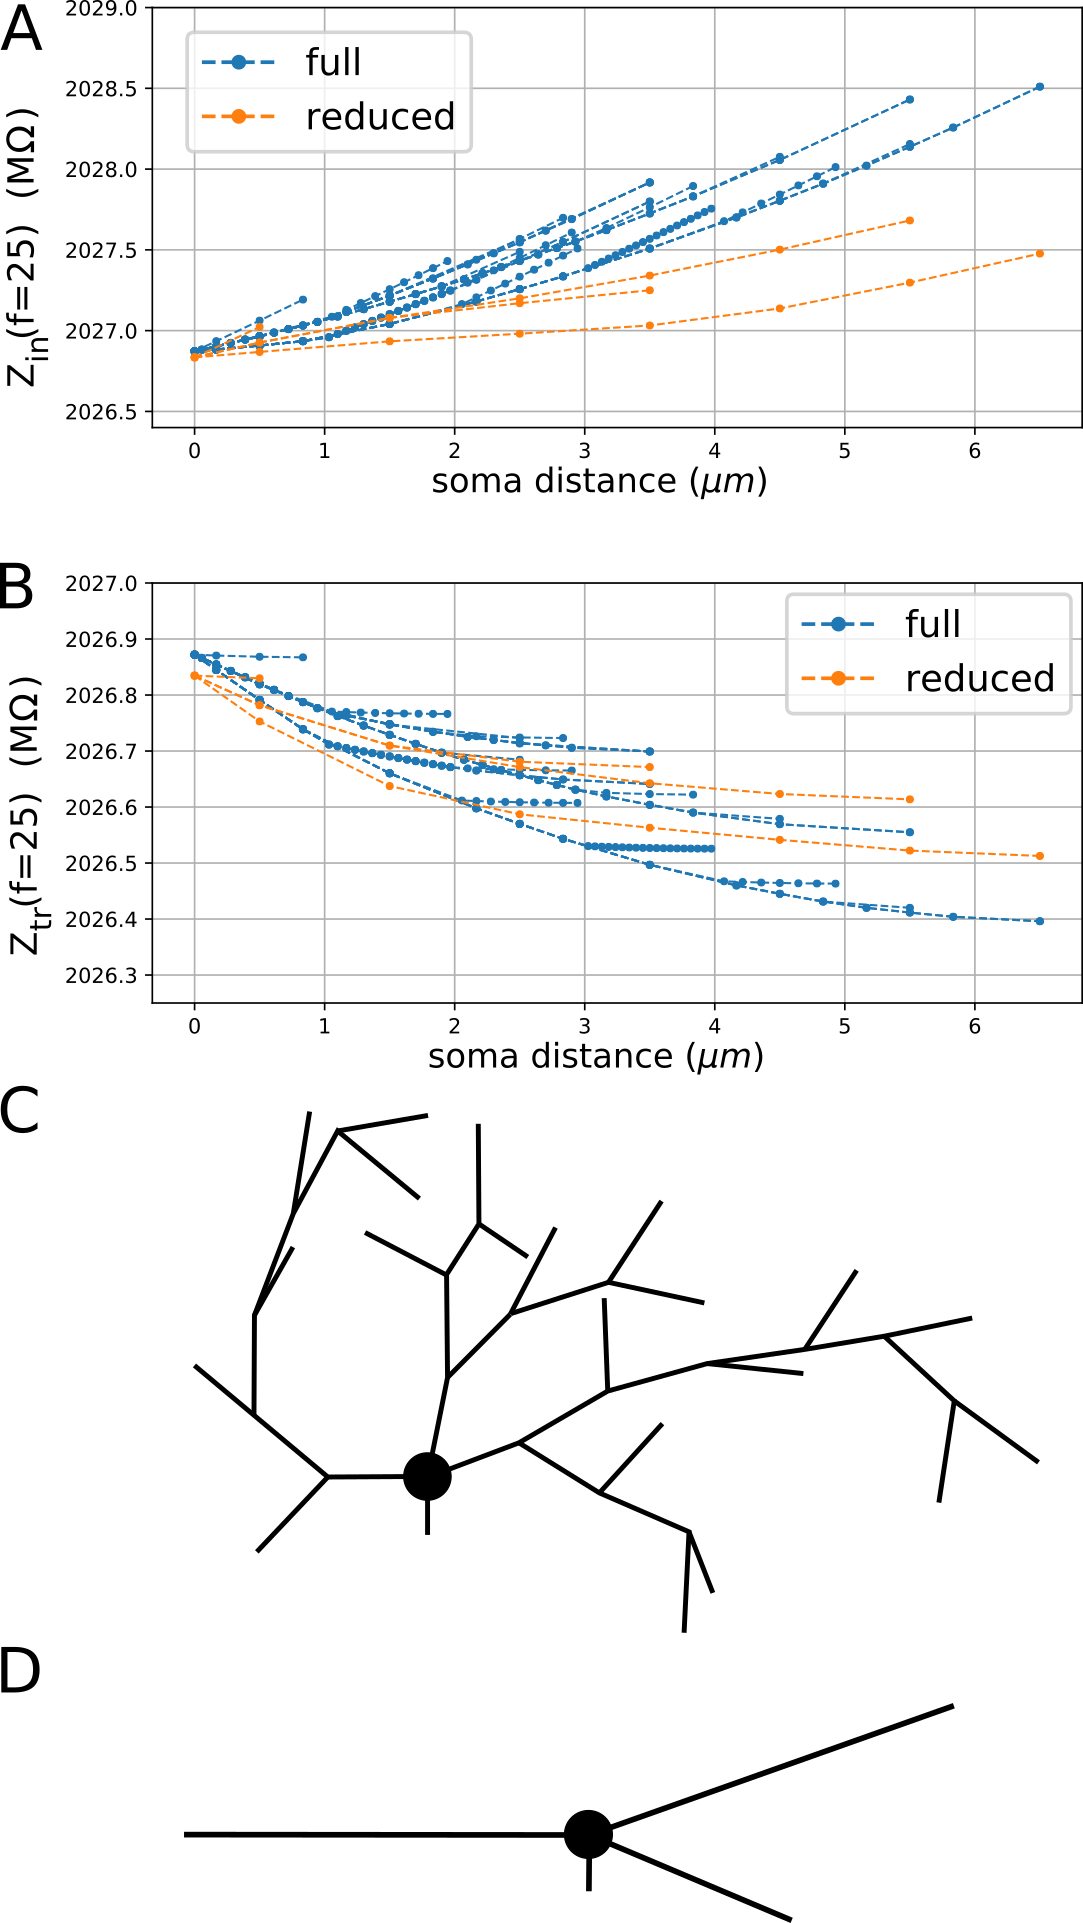
\includegraphics[height=\dimexpr \textheight - 9\baselineskip\relax]{ch_reduced_model/figs/fig_gpe-full-vs-red_Zin-Ztr.png}
\caption{
\textbf{Morphological and electrical characteristics of detailed and reduced GPe neuron models.}
\textbf{A}: Local input impedance seen at different points in the dendritic tree, as a function
of distance from the soma.
\textbf{B}: Local transfer impedance to the soma for current sources located at different points
in the dendritic tree.
\textbf{C}: Schematic diagram of the detailed STN neuron morphology. Paths along dendrites where
input and transfer impedances were measured are highlighted in blue.
\textbf{D}: Schematic diagram of the reduced STN neuron morphology. Dendrites are represented by
three equivalent cylinders. Paths where input and transfer impedances were measured are highlighted
in orange.
}
\label{fig:gpe-full-vs-red_Zin-Ztr}
\end{figure}

%
%
%
\subsection{Stereotypical responses of neuron models}
%
%
%
%
%
%
%
%
%

%
%
%

%
%
%

%
%
%
%
%
%
%
%
%
%
%

Comparing the responses of detailed and reduced STN and GPe models to current
clamp protocols designed to elicit stereotypical responses show that these
are well captured by the reduced cell models (Fig.~\ref{fig:stn-full-vs-red_protos-clamp} - \ref{fig:gpe-full-vs-red_protos-clamp}).

%
%
%
%
%
%
%
%
%
%
%
%
%
%
%
%
%
STN model neurons fire spontaneously at approximately 9 Hz (Fig.~\ref{fig:stn-full-vs-red_protos-clamp}.Ai - Aii), capturing their
behavior in vitro where they fire between 5-15 Hz \cite{gillies_membrane_2005}),
mediated by the persistent sodium current (NaP channel).
Both STN neuron models show a rebound burst response in response to offset of
hyperpolarizing current (Fig.~\ref{fig:stn-full-vs-red_protos-clamp}.Bi, Bii),
and a plateau potential in response to a depolarizing input delivered while the
cell is hyperpolarized (Fig.~\ref{fig:stn-full-vs-red_protos-clamp}.Ci, Cii).
%
%
%

%

%
The automatic reduction method preserved the stereotypical responses well without
manual fine tuning of parameters. The spontaneous firing rate was 12.5\% lower in the
reduced model compared to the original cell model. This could be rectified by increasing
the density of the persistent sodium (NaP) current in the reduced cell model by 1.7\%.
The rebound burst response was preserved, but its length was reduced from 17 to 10 spikes
caused by earlier termination of $Ca^{2+}$ influx in dendritic ion channels.
%
%
%
%
The plateau potential (Fig.~\ref{fig:stn-full-vs-red_protos-clamp}.C) was also preserved
in the reduced model but shortened in duration by one spike, as its underlying
currents are the same as those for the rebound burst.
%
%
%

\begin{figure}[ht]
\centering
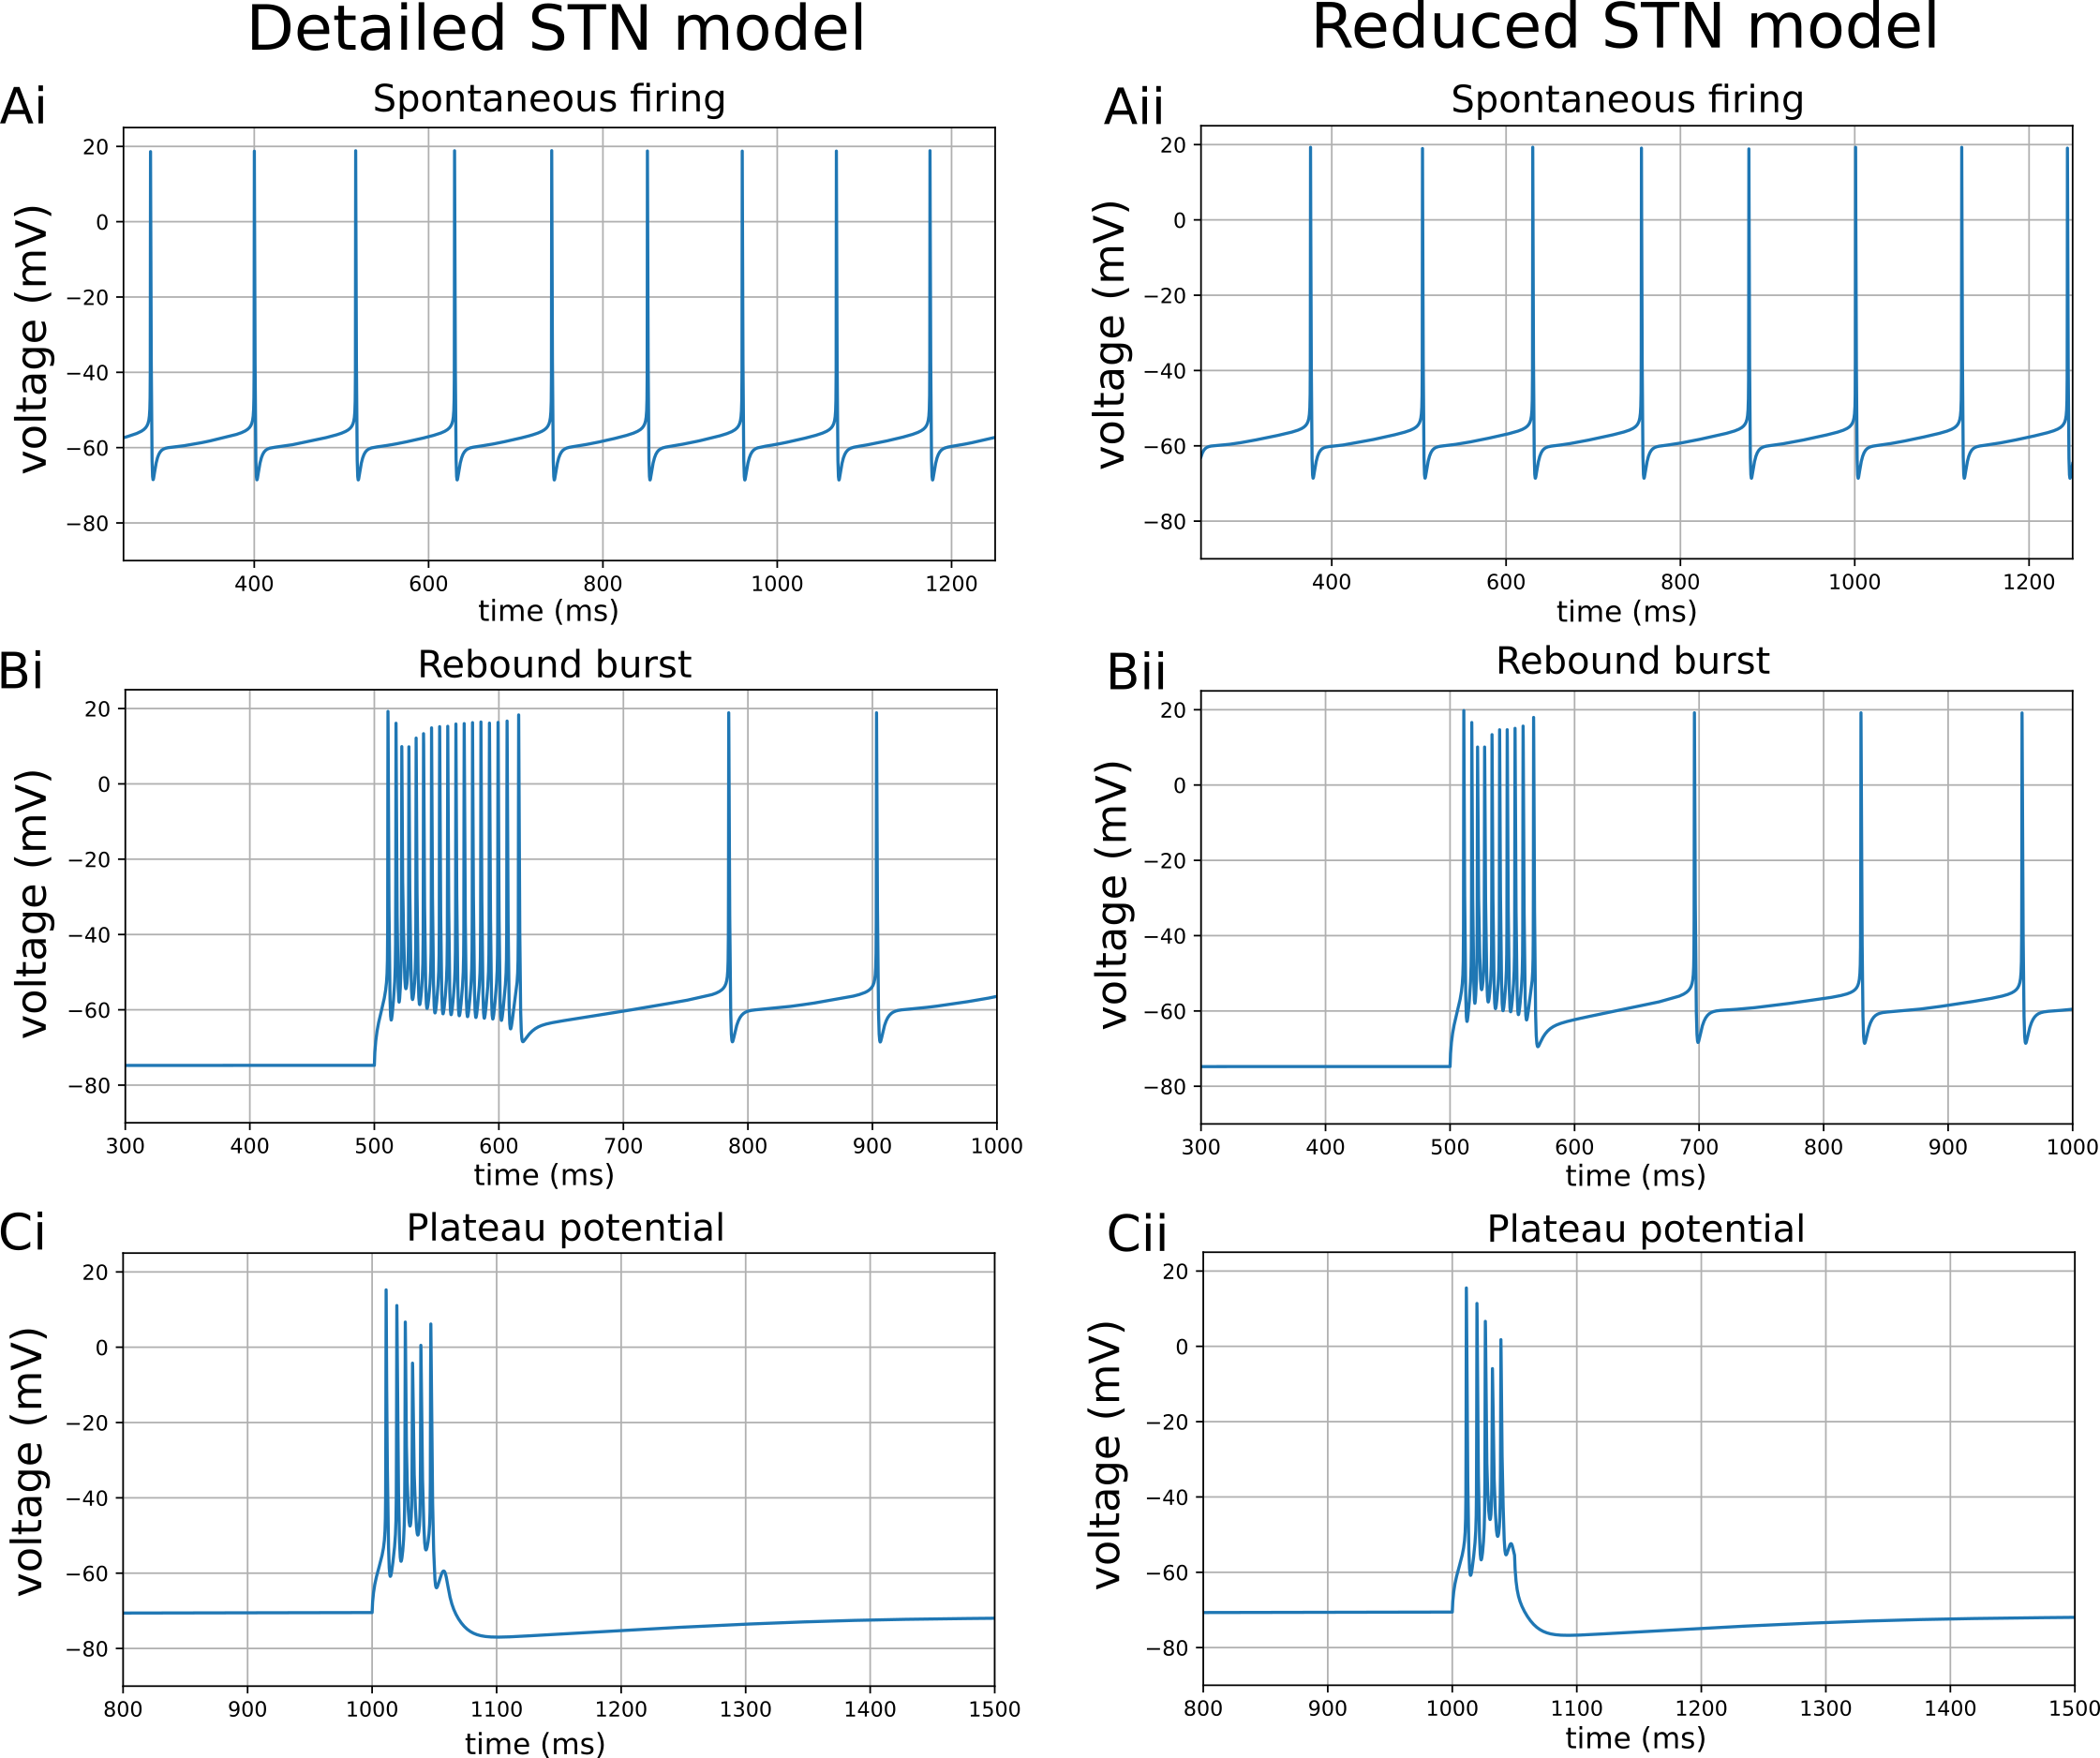
\includegraphics[width=\textwidth]{ch_reduced_model/figs/fig_stn-full-vs-red_protos-clamp.png}
\caption{\textbf{Stereotypical responses of the \cite{gillies_membrane_2005} STN neuron model recorded in detailed and reduced cell models.}
Responses of the detailed and reduced cell models are shown in column i and ii, respectively.
\textbf{A}: Spontaneous firing in absence of stimulation. Firing rate is 9.14 Hz in original cell model
and 8.0 Hz in reduced cell model.
\textbf{B}: Rebound burst response. Burst is shortened from 17 to 10 spikes in reduced cell model.
\textbf{C}: Plateau potential activated at hyperpolarized potentials. Number of spikes on the plateau
is reduced by one in the reduced cell model.}
\label{fig:stn-full-vs-red_protos-clamp}
\end{figure}

%
%

GPe neurons in vitro fire spontaneously at 15 Hz with a characteristic
action potential shape \cite{gunay_channel_2008}, which was well captured by the
detailed and reduced model neurons (Fig.~\ref{fig:gpe-full-vs-red_protos-clamp}.Ai, Aii).
%
Other features of GPe projection neurons that were captured with high precision by the original
model neuron \cite{gunay_channel_2008} and the reduced model are rapid firing (36 Hz)
with spike height adaptation in response to a positive current pulse
(100 pA, Fig.~\ref{fig:gpe-full-vs-red_protos-clamp}.Bi, Bii),
and a characteristic sag in the membrane voltage in response to hyperpolarizing current
(-100 pA), mediated by HCN current (Fig.~\ref{fig:gpe-full-vs-red_protos-clamp}.Ci, Cii).

\begin{figure}[ht]
\centering
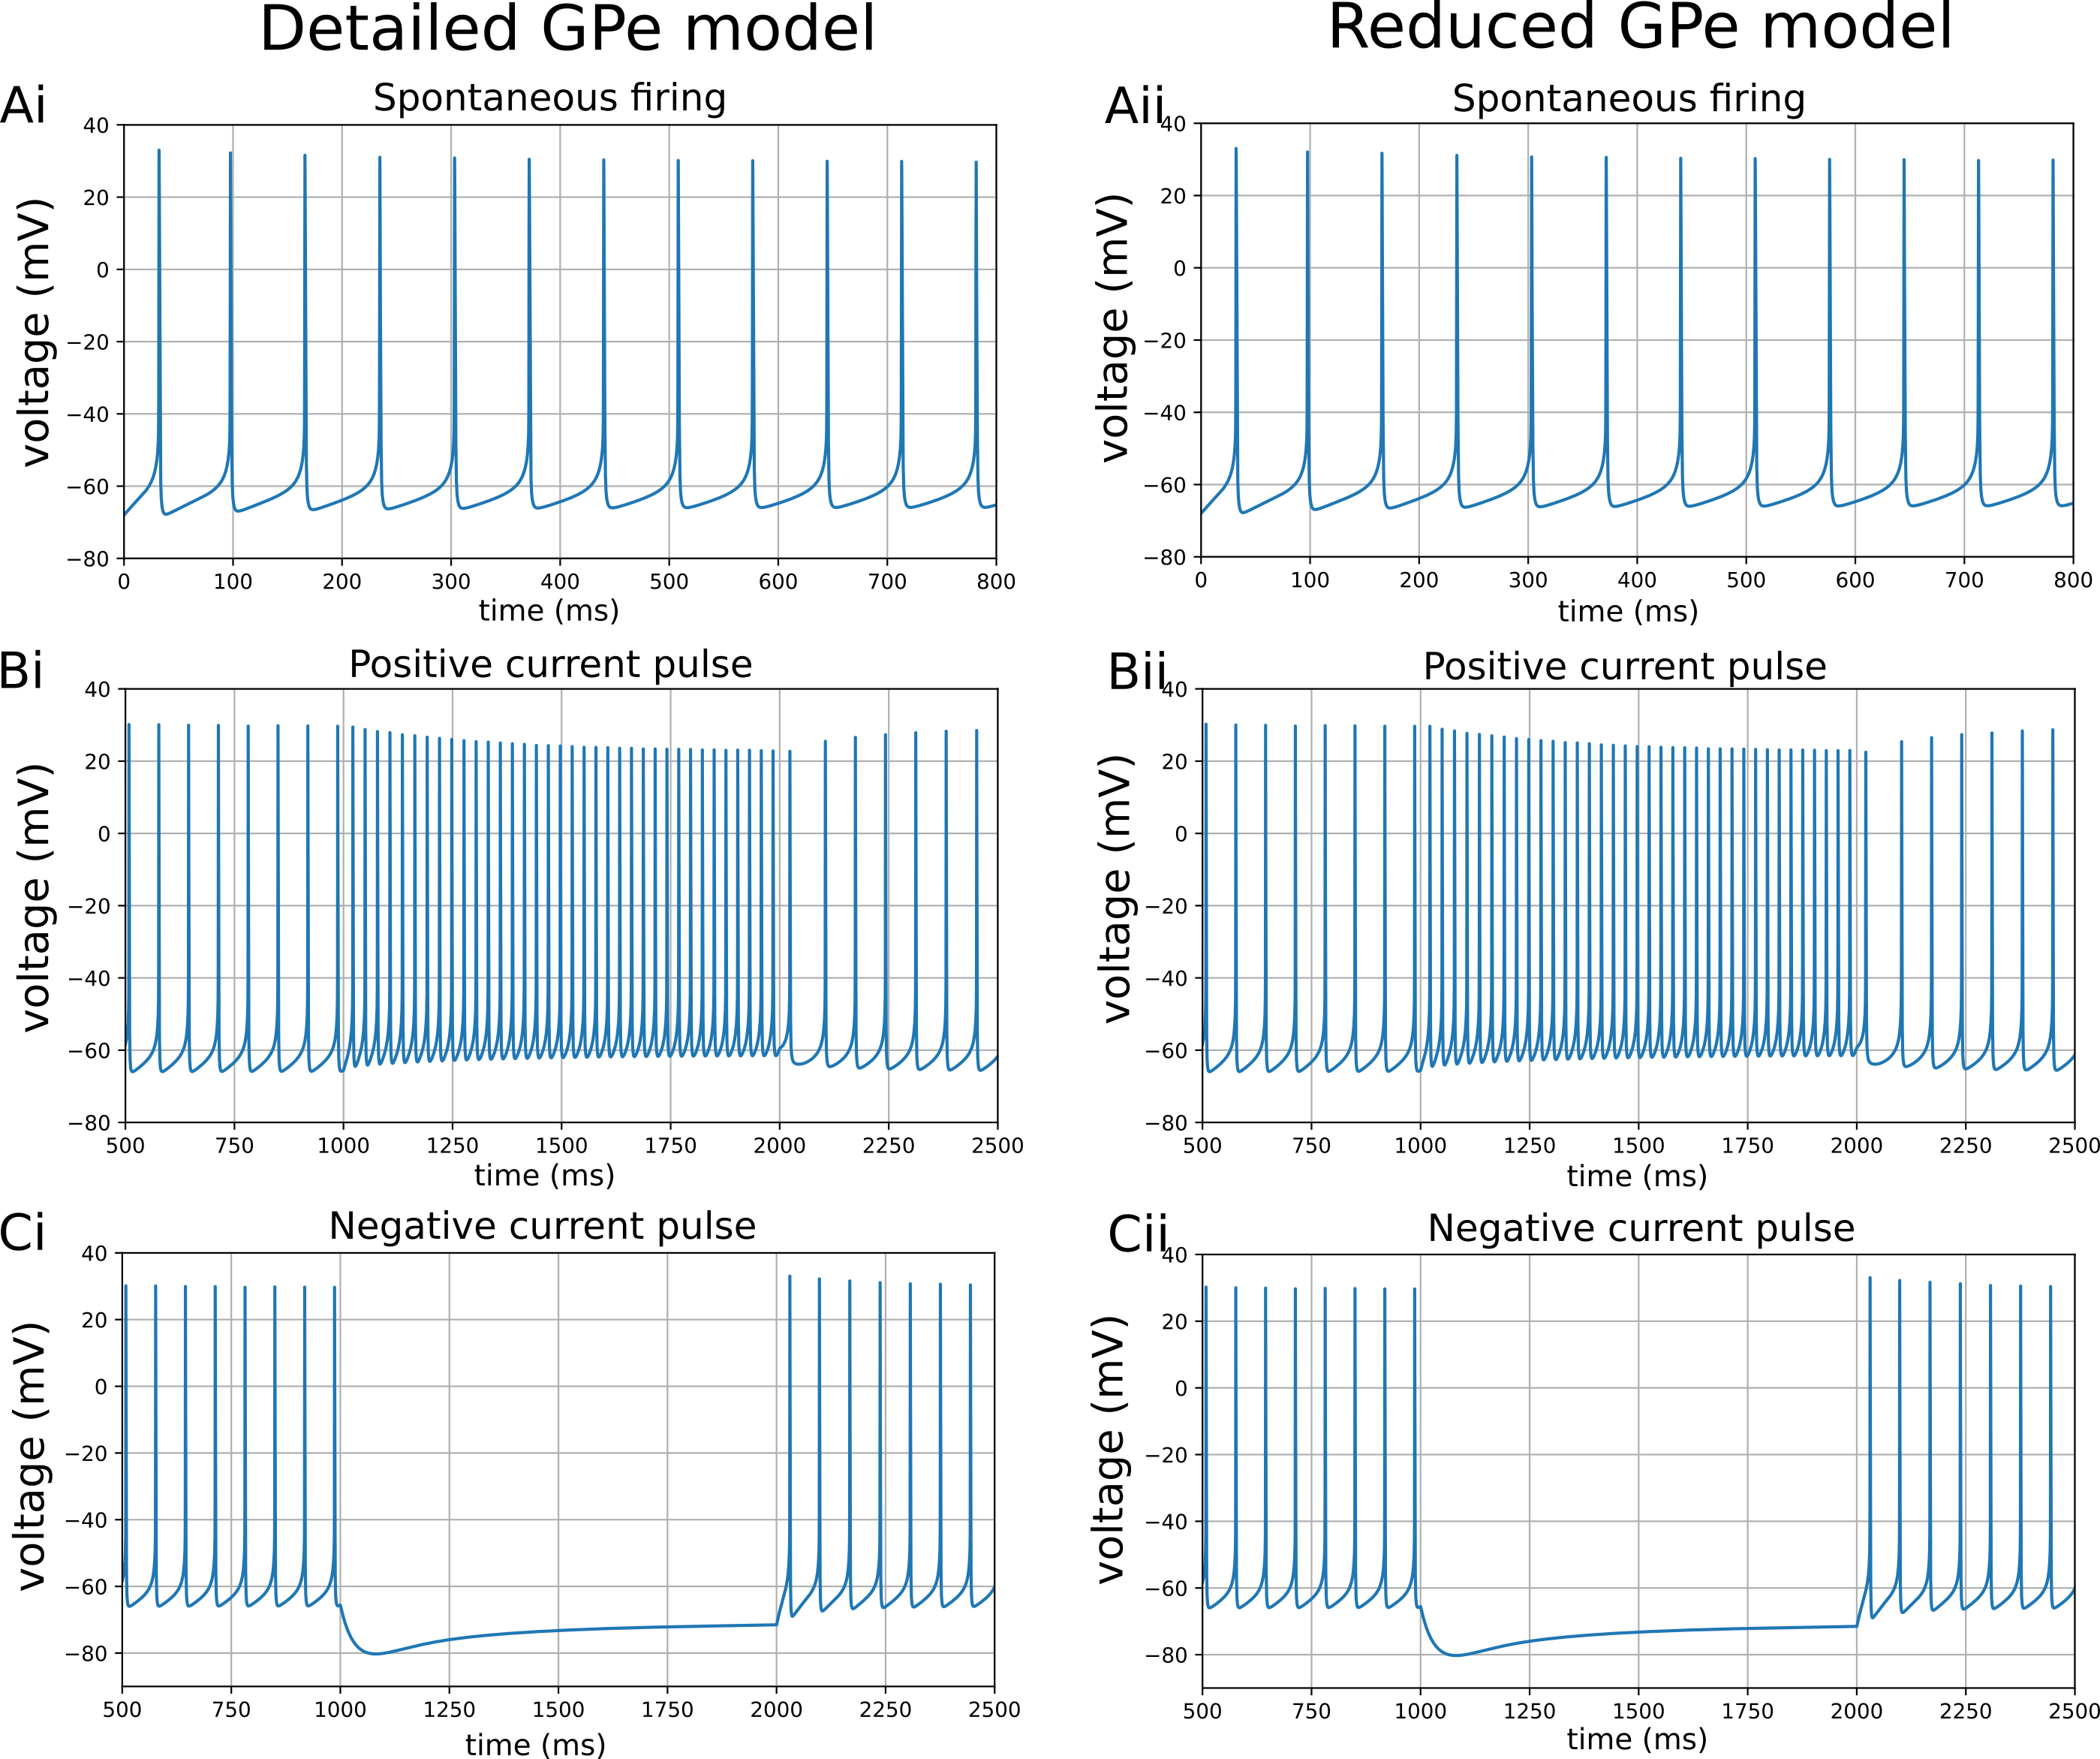
\includegraphics[width=\textwidth]{ch_reduced_model/figs/fig_gpe-full-vs-red_protos-clamp.png}
\caption{
\textbf{Stereotypical responses of the \cite{gunay_channel_2008} GPe neuron model recorded in detailed and reduced cell models.}
Responses of the detailed and reduced cell models are shown in column i and ii, respectively.
\textbf{A}: Spontaneous firing in absence of stimulation. Firing rate is 15 Hz in both models.
\textbf{B}: Spike height adaptation during positive current injection.
\textbf{C}: Characteristic sag mediated by HCN current during negative current injection.
}
\label{fig:gpe-full-vs-red_protos-clamp}
\end{figure}

%
%
%
\subsection{Neuronal synchronization properties characterized by phase response curves}
%
%
%
%
%
%
%

%
%

To measure how the detailed and reduced models synchronized to their synaptic inputs, PRC
were measured using synaptic inputs located at biologically realistic locations
in the cells' dendritic trees (Ch.~\ref{sec:ch3-methods}, Fig.~\ref{fig:network_diagram}).
%
%

%
In the STN neuron models, excitatory PRC were positive for synaptic inputs
arriving in the middle segment of the ISI and had smaller negative regions
near the start and end of the ISI (Fig.~\ref{fig:stn-full-vs-red_PRC-curves}.A, B). %
Although small negative regions at the start of the ISI are commonly permitted in
classification of type I PRC, due to stimulation during the downstroke of the
action potential, the negative region at the end of the ISI indicates a type II PRC.
When the excitatory synapse was placed farther down the dendrite, more distally to the soma,
the negative region at the end of the ISI became larger and covered a larger phase
interval and the magnitude of the phase shift was reduced. This vertical scaling
of the PRC as the synapse is moved to a more distant location in the dendrite
reflects increased attenuation of post-synaptic potentials originating at distant
sites.
%
Excitatory PRCs were well preserved in the reduced cell model
(Fig.~\ref{fig:stn-full-vs-red_PRC-curves}.Aii, Bii), with only small deviation
between polynomial fits to the PRC samples.
%
Inhibitory PRC were negative for synaptic inputs arriving in the middle segment
of the ISI and had positive regions at the start and end of the ISI
(Fig.~\ref{fig:stn-full-vs-red_PRC-curves}.C). Phase shifts elicited by stimuli
arriving late in the ISI showed a large variance, reflecting a large residual
influence of past stimuli on ion channels governing the membrane voltage. %
This was the case in both the detailed and reduced cell model, resulting
in a larger mismatch between PRC for later phases, while the match in early
phases was close (Fig.~\ref{fig:stn-full-vs-red_PRC-curves}.C).

\begin{figure}[ht]
\centering
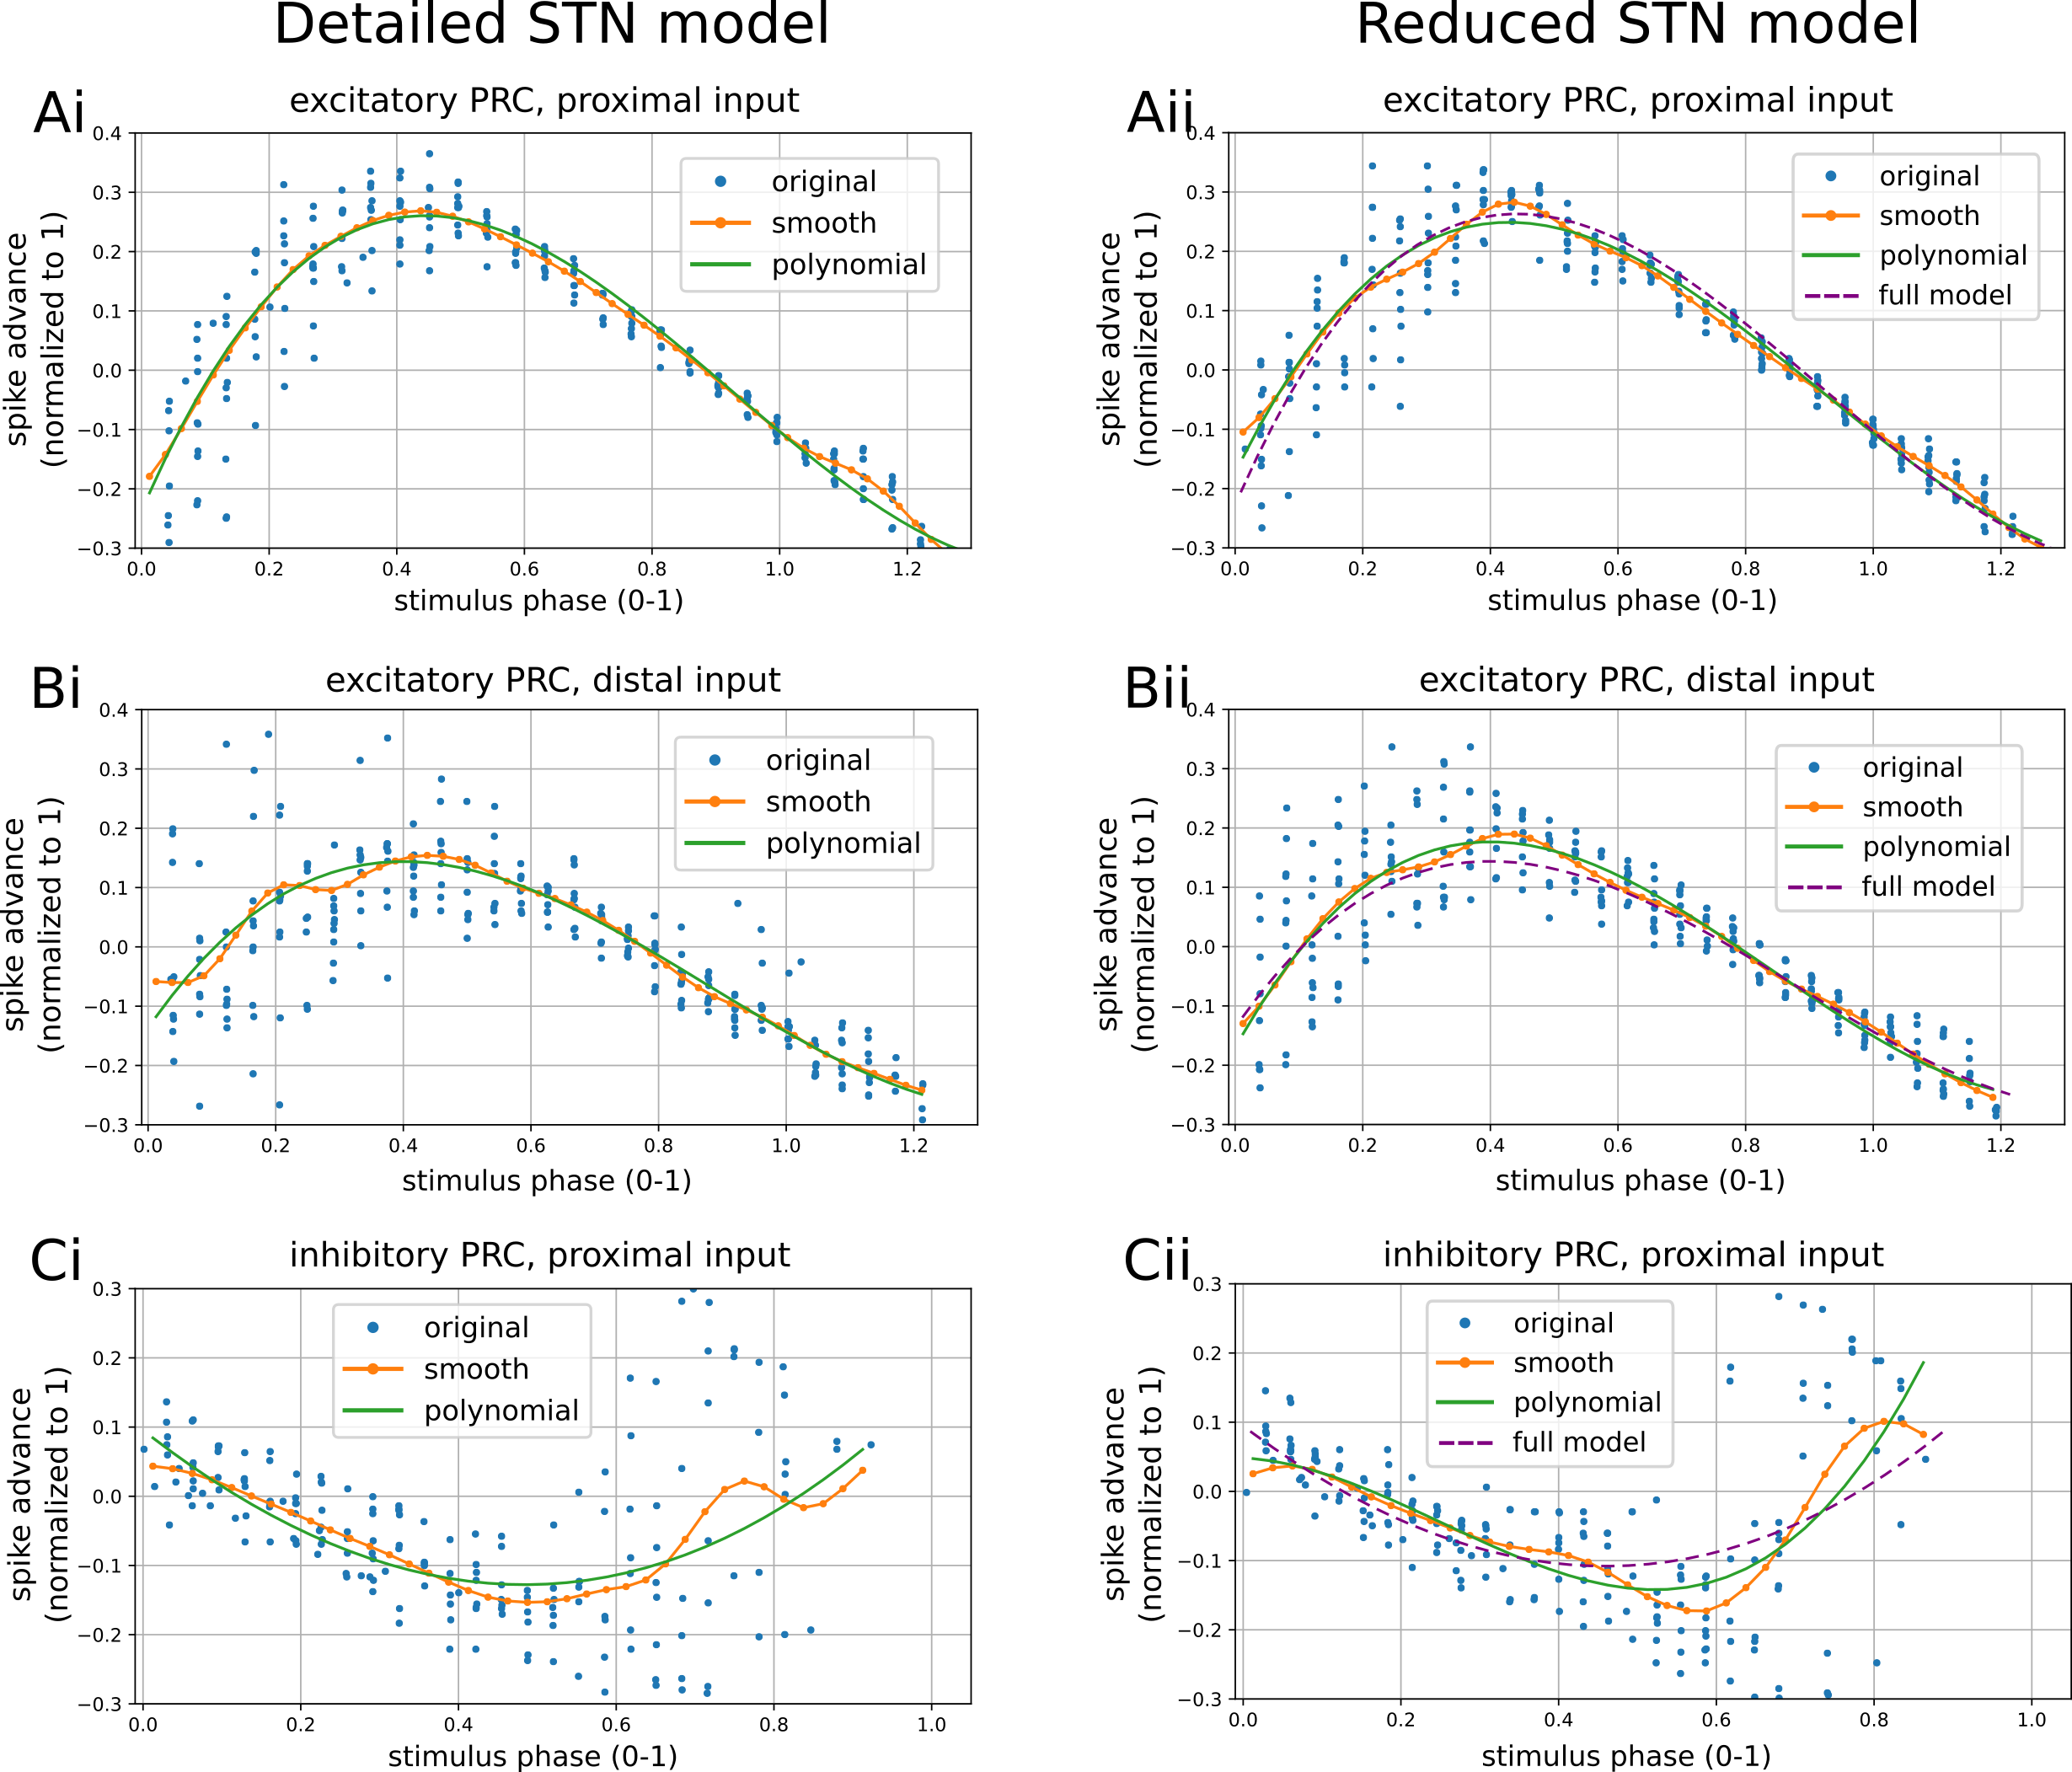
\includegraphics[width=\textwidth]{ch_reduced_model/figs/fig_stn-full-vs-red_PRC-curves.png}
\caption{\textbf{Phase response curves of detailed and reduced GPe neurons in response to synaptic inputs.}
PRC of detailed and reduced cell models are shown in column i and ii, respectively.
\textbf{A}: PRC in response to excitatory synaptic inputs located distally in the dendritic tree.
\textbf{B}: PRC in response to inhibitory synaptic inputs located proximally to the soma.
\textbf{C}: PRC in response to excitatory synaptic inputs located proximally in the dendritic tree.}
\label{fig:stn-full-vs-red_PRC-curves}
\end{figure}

%
%

In the GPe neuron model, excitatory dendritic PRCs were clearly biphasic with a large
negative region starting at the last 30th percentile of the ISI
(Fig.~\ref{fig:gpe-full-vs-red_PRC-curves}.A, B).
The inhibitory PRC was largely symmetric with the excitatory one, showing a large negative
region followed by a smaller positive region in the last 40th - 30th percentile.
Both types of PRC were again well matched by the reduced GPe model (Fig.~\ref{fig:gpe-full-vs-red_PRC-curves}.Aii, Bii, Cii),
indicating that the phase response was preserved between the two models.

\begin{figure}[ht]
\centering
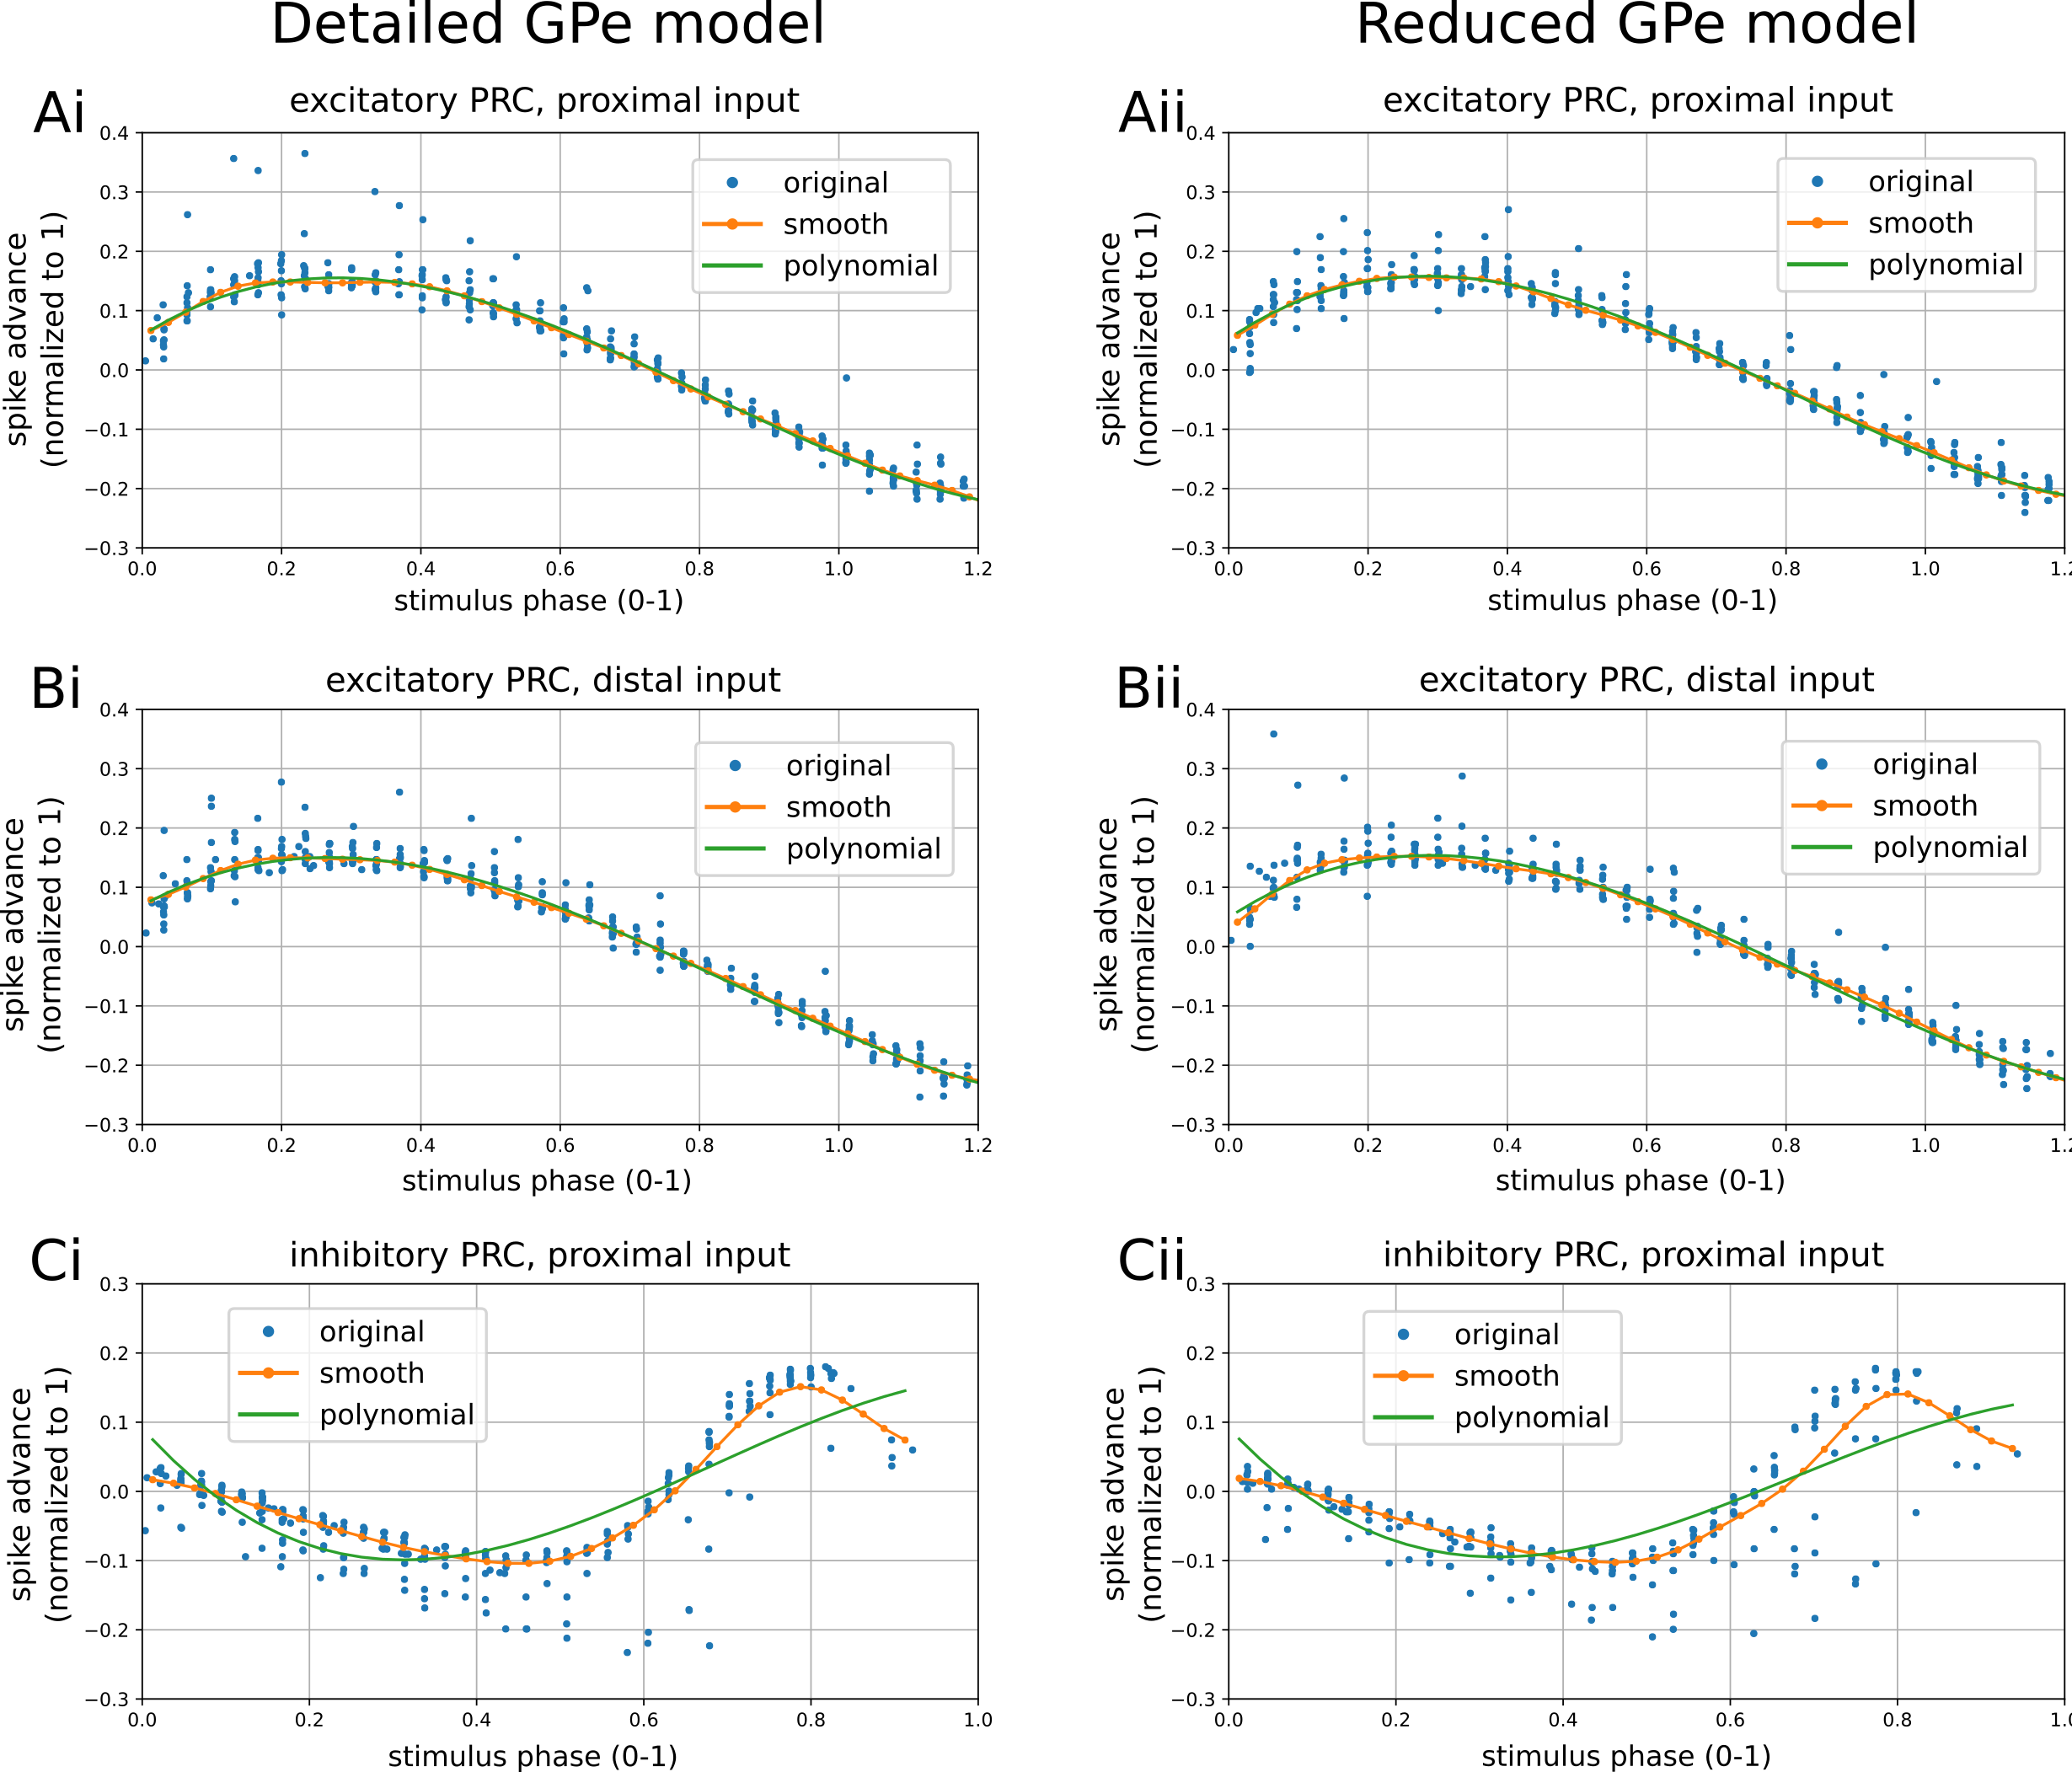
\includegraphics[width=\textwidth]{ch_reduced_model/figs/fig_gpe-full-vs-red_PRC-curves.png}
\caption{\textbf{Phase response curves of detailed and reduced GPe neurons in response to synaptic inputs.}
PRC of detailed and reduced cell models are shown in column i and ii, respectively.
\textbf{A}: PRC in response to excitatory synaptic inputs located distally in the dendritic tree.
\textbf{B}: PRC in response to inhibitory synaptic inputs located proximally to the soma.
\textbf{C}: PRC in response to excitatory synaptic inputs located proximally in the dendritic tree.}
\label{fig:gpe-full-vs-red_PRC-curves}
\end{figure}

%
%
%
%

%
%
%
\subsection{Simulation of the STN-GPe network using reduced cell models}
%

%
%

In order to assess the effectiveness of the reduced cell models to capture
the characteristics of the original neuron models essential to their
network behavior, the cell models were substituted in the network model of the
STN-GPe loop presented in Chapter~\ref{ch3:detailed-model} and network activity
and firing patterns were compared. The frequency response of both networks
in the beta-band in particular was investigated. Given the correlation
between the improvement in Parkinsonian motor symptoms and the suppression
of beta-band oscillatory activity in the STN-GPe network
\cite{kuhn_reduction_2006,weinberger_beta_2006,eusebio_deep_2011,ray_local_2008},
the frequency response in this band should be maintained in the reduced network if the model is
to be used to optimize DBS stimulation prototocols.

%
%

%
%
%
%
The first key behavior exhibited by the detailed network model of Chapter~\ref{ch3:detailed-model}
was its ability to show weak spontaneous oscillations in the beta-band range with the
oscillation frequency depending on degree of excitation by cortical inputs
(Fig.~\ref{fig:endogenous_sweep-gmax-ctx-stn_A-psd-currents}, \ref{fig:endogenous_sweep-gaba-AB-gpe-stn_AC-psd-all}).
This behavior was retained in the reduced network model, with differences observed
in the power of beta-band and low-frequency (2-5 Hz) oscillations
(Fig.~\ref{fig:net-full-vs-red_spont_sweep-g-ctx-stn}).

In the detailed network model, increasing the strength of cortical excitation
revealed a parameter region at intermediate synaptic strengths where strong
low-frequency bursting (2-5 Hz) in the STN co-occurred with weak synchronization
(Fig.~\ref{fig:net-full-vs-red_spont_sweep-g-ctx-stn}, $ 0.4 < gmax < 0.9 $).
Although this parameter region is present in the reduced network model,
the power of low-frequency oscillations is lower (Fig.~\ref{fig:net-full-vs-red_spont_sweep-g-ctx-stn},
right column). The reduction in low-frequency power was related to the fact
that the reduced STN neuron models were less prone to bursting
(Fig.~\ref{fig:net-full-vs-red_spont_sweep-g-ctx-stn}.C): with a synaptic
strength corresponding to the maximum low-frequency power ($gmax_{CTX-STN} = 0,7$)
in the detailed model, STN neurons showed a mean burst rate of 0.5 bursts/sec
in the reduced model compared to 1.5 bursts/sec in the detailed model.
%

\begin{figure}[ht]
\centering
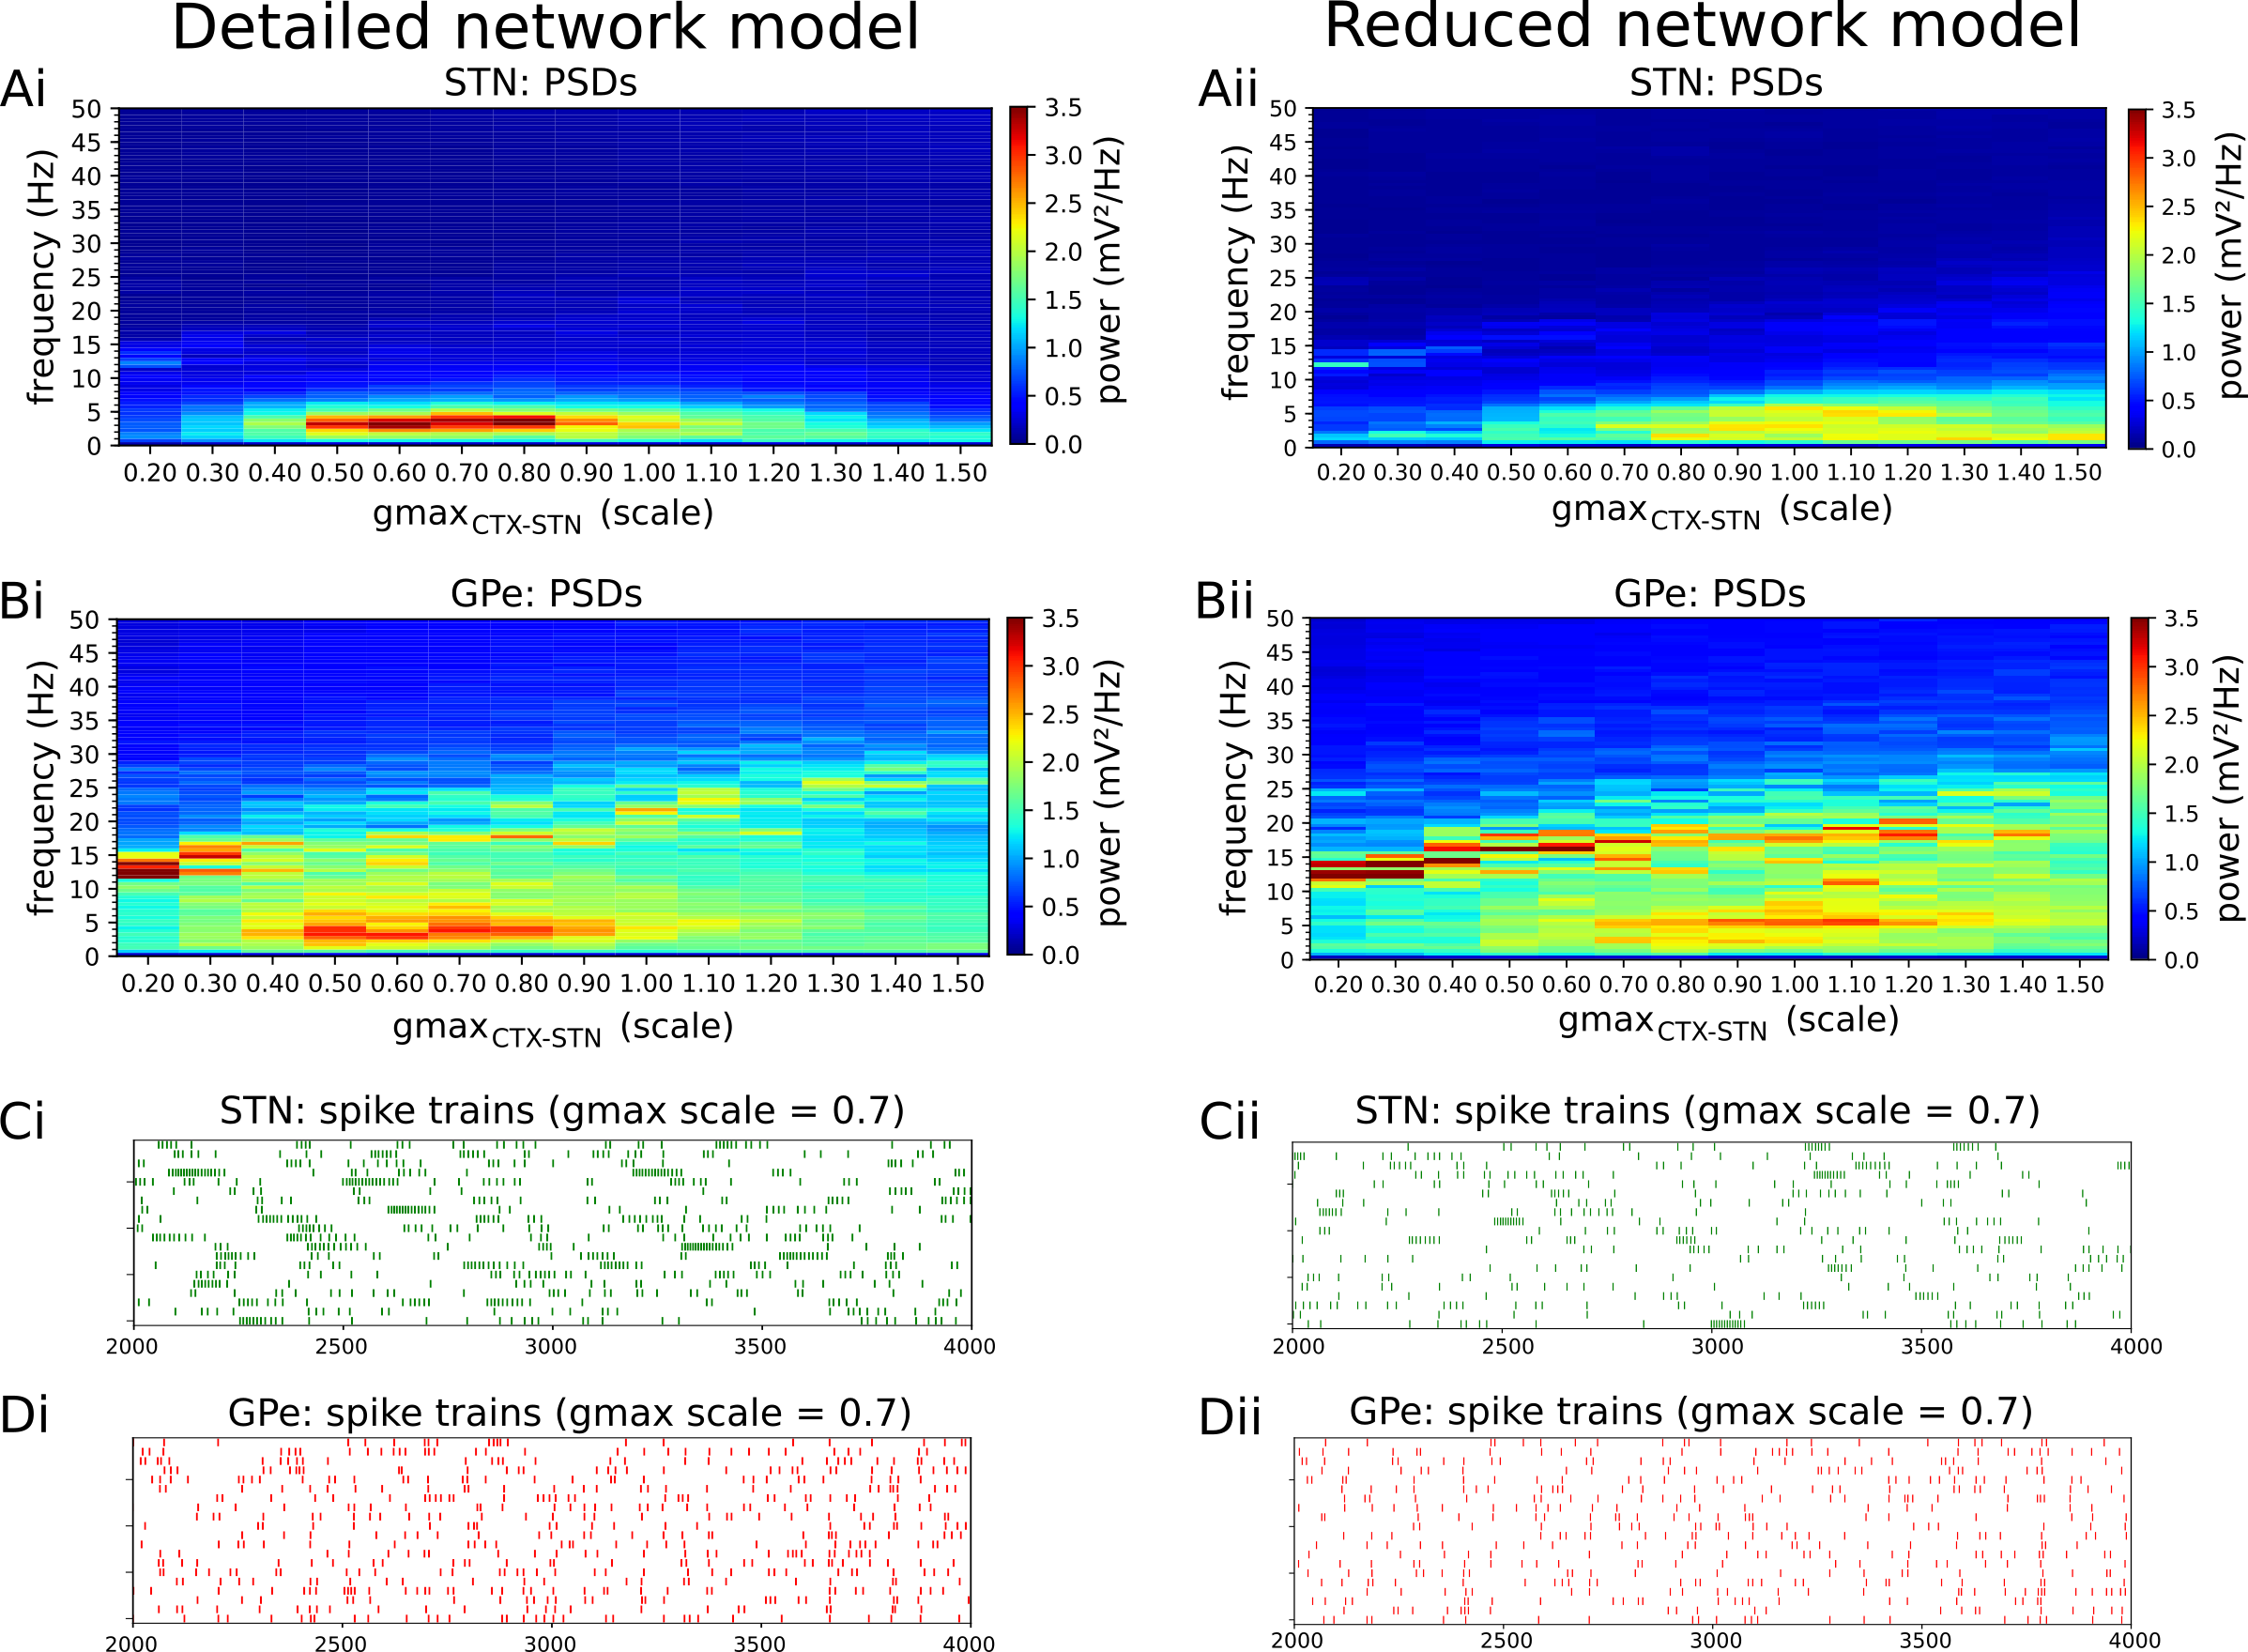
\includegraphics[width=\textwidth]{ch_reduced_model/figs/fig_net-full-vs-red_sweep-g-ctx-stn_spont.png}
\caption{
\textbf{Effect of cortical excitation on firing patterns and oscillation frequency in the STN-GPe network.}
Power spectral densities and spike raster plots for the detailed network model (column i, left) and network using reduced neuron models (column ii, right). Mean power spectral density (PSD) of somatic membrane voltages of STN neurons \textbf{(A)} and GPe neurons \textbf{(B)}. Representative spike trains for STN \textbf{(C)} and GPe population \textbf{(D)} for intermediate level of cortical excitation corresponding to low-frequency bursting regimen.
}
\label{fig:net-full-vs-red_spont_sweep-g-ctx-stn}
\end{figure}

%
%

The second key behavior of the detailed network model was resonance of the STN-GPe feedback loop
with cortical beta-band activity arriving via CTX-STN afferents.
The resonance behavior was qualitatively retained by the reduced network model
(Fig.~\ref{fig:net-full-vs-red_sweep-f-burst}) but the resonance peaks in the STN and GPe
populations were shifted toward the lower frequency range by approximately 6 Hz (Fig.~\ref{fig:net-full-vs-red_sweep-f-burst}.C,D) and increased in magnitude.
%
The phase vector lengths were also increased (Fig.~\ref{fig:net-full-vs-red_sweep-f-burst}.C),
indicating stronger phase synchronization to the cortical oscillation in STN and GPe spike trains.
This occurred despite the close match in phase response curves, indicating that
PRC alone are not a good predictor of synchronization strength. For example, between 15-18 Hz
there is a large discrepancy in the strength of phase synchronization between the full
and reduced models. This discrepancy could be explained, however, by differences in
excitability and firing rates between the two models:
the decrease in resonance frequency and increase in resonance strength was
accompanied by lower firing rates in STN neurons but not in GPe neurons (Fig.~\ref{fig:net-full-vs-red_sweep-f-burst_currents-EI}.C). Moreover, the
total synaptic currents delivered to STN and GPe neurons were decreased (Fig.~\ref{fig:net-full-vs-red_sweep-f-burst_currents-EI}.A-B, shaded areas).

The downward shift in resonance frequency in the reduced model mirrors the
results of Chapter~\ref{ch3:detailed-model} where the the frequency of maximal
phase locking decreases with the ratio of excitation to inhibition and the strength
of phase locking increases (Fig.~\ref{fig:exogenous_ctx-resonance-response_B-vectorlength}.B-C).
Although STN neurons in the reduced model have a lower firing rate and the net
synaptic current is smaller in the frequency range of resonance, the estimated E/I ratio is not
consistently lower (Fig.~\ref{fig:net-full-vs-red_sweep-f-burst_currents-EI}.A).
%
This paradoxical observation could be due to inaccurate estimation of the E/I ratio
based on recordings in only 6 \% of cells or it could be due to the increased effectiveness
of inhibition in the electrically compact reduced neuron model.
%
%
%
%
%
%
%
%
%
%
%
%

\begin{figure}[ht]
\centering
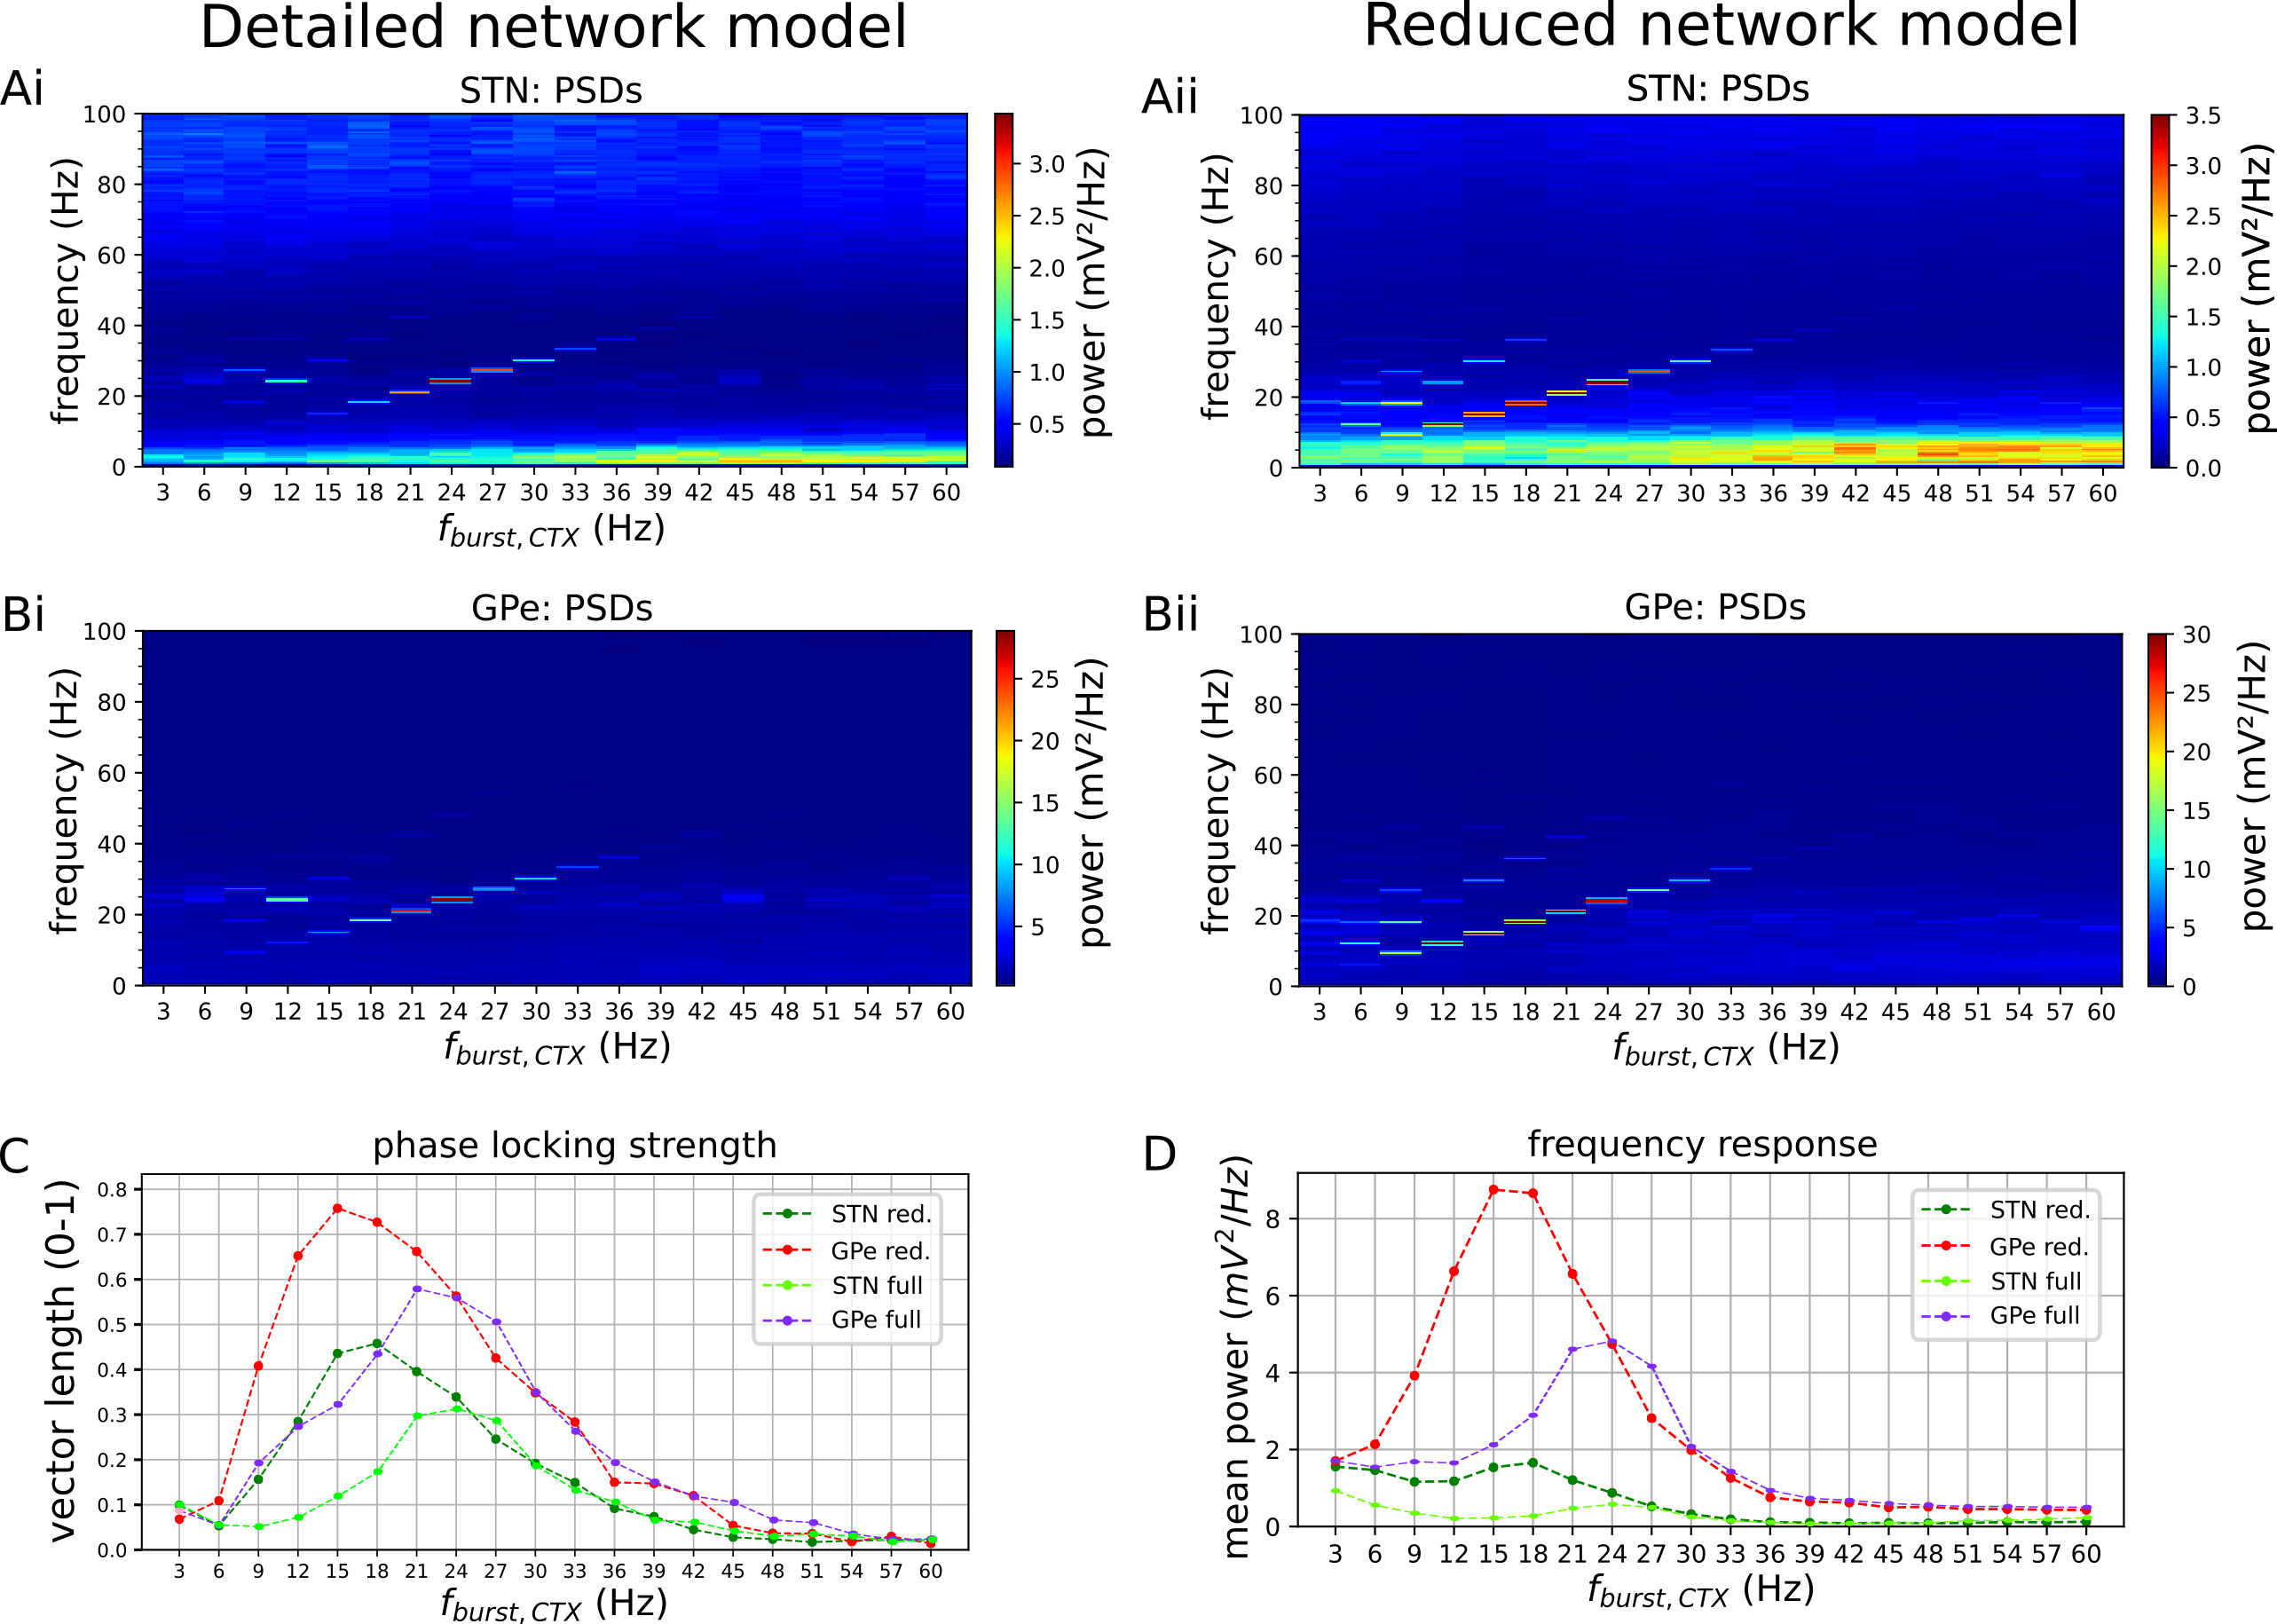
\includegraphics[width=\textwidth]{ch_reduced_model/figs/fig_net-full-vs-red_sweep-f-burst-ctx.png}
\caption{
\textbf{Frequency response and phase locking of the STN-GPe network to cortical oscillatory bursting inputs.}
\textbf{A,B}: Mean power spectral density (PSD) of somatic membrane voltages of STN neurons \textbf{(A)} and GPe neurons \textbf{(B)} for the detailed network model (column i, left) and network using reduced neuron models
(column ii, right).
\textbf{C}: Population vector length, indicating strength of phase locking to cortical oscillations of increasing frequencies. Detailed network model in dark green, red for STN, GPe respectively. Reduced model in bright green, purple for STN, GPe respectively.
\textbf{D}: Frequency response of the STN and GPe populations, measured by taking the mean PSD values in a 5 Hz window centered on the cortical oscillation frequency.
}
\label{fig:net-full-vs-red_sweep-f-burst}
\end{figure}

\begin{figure}[ht]
\centering
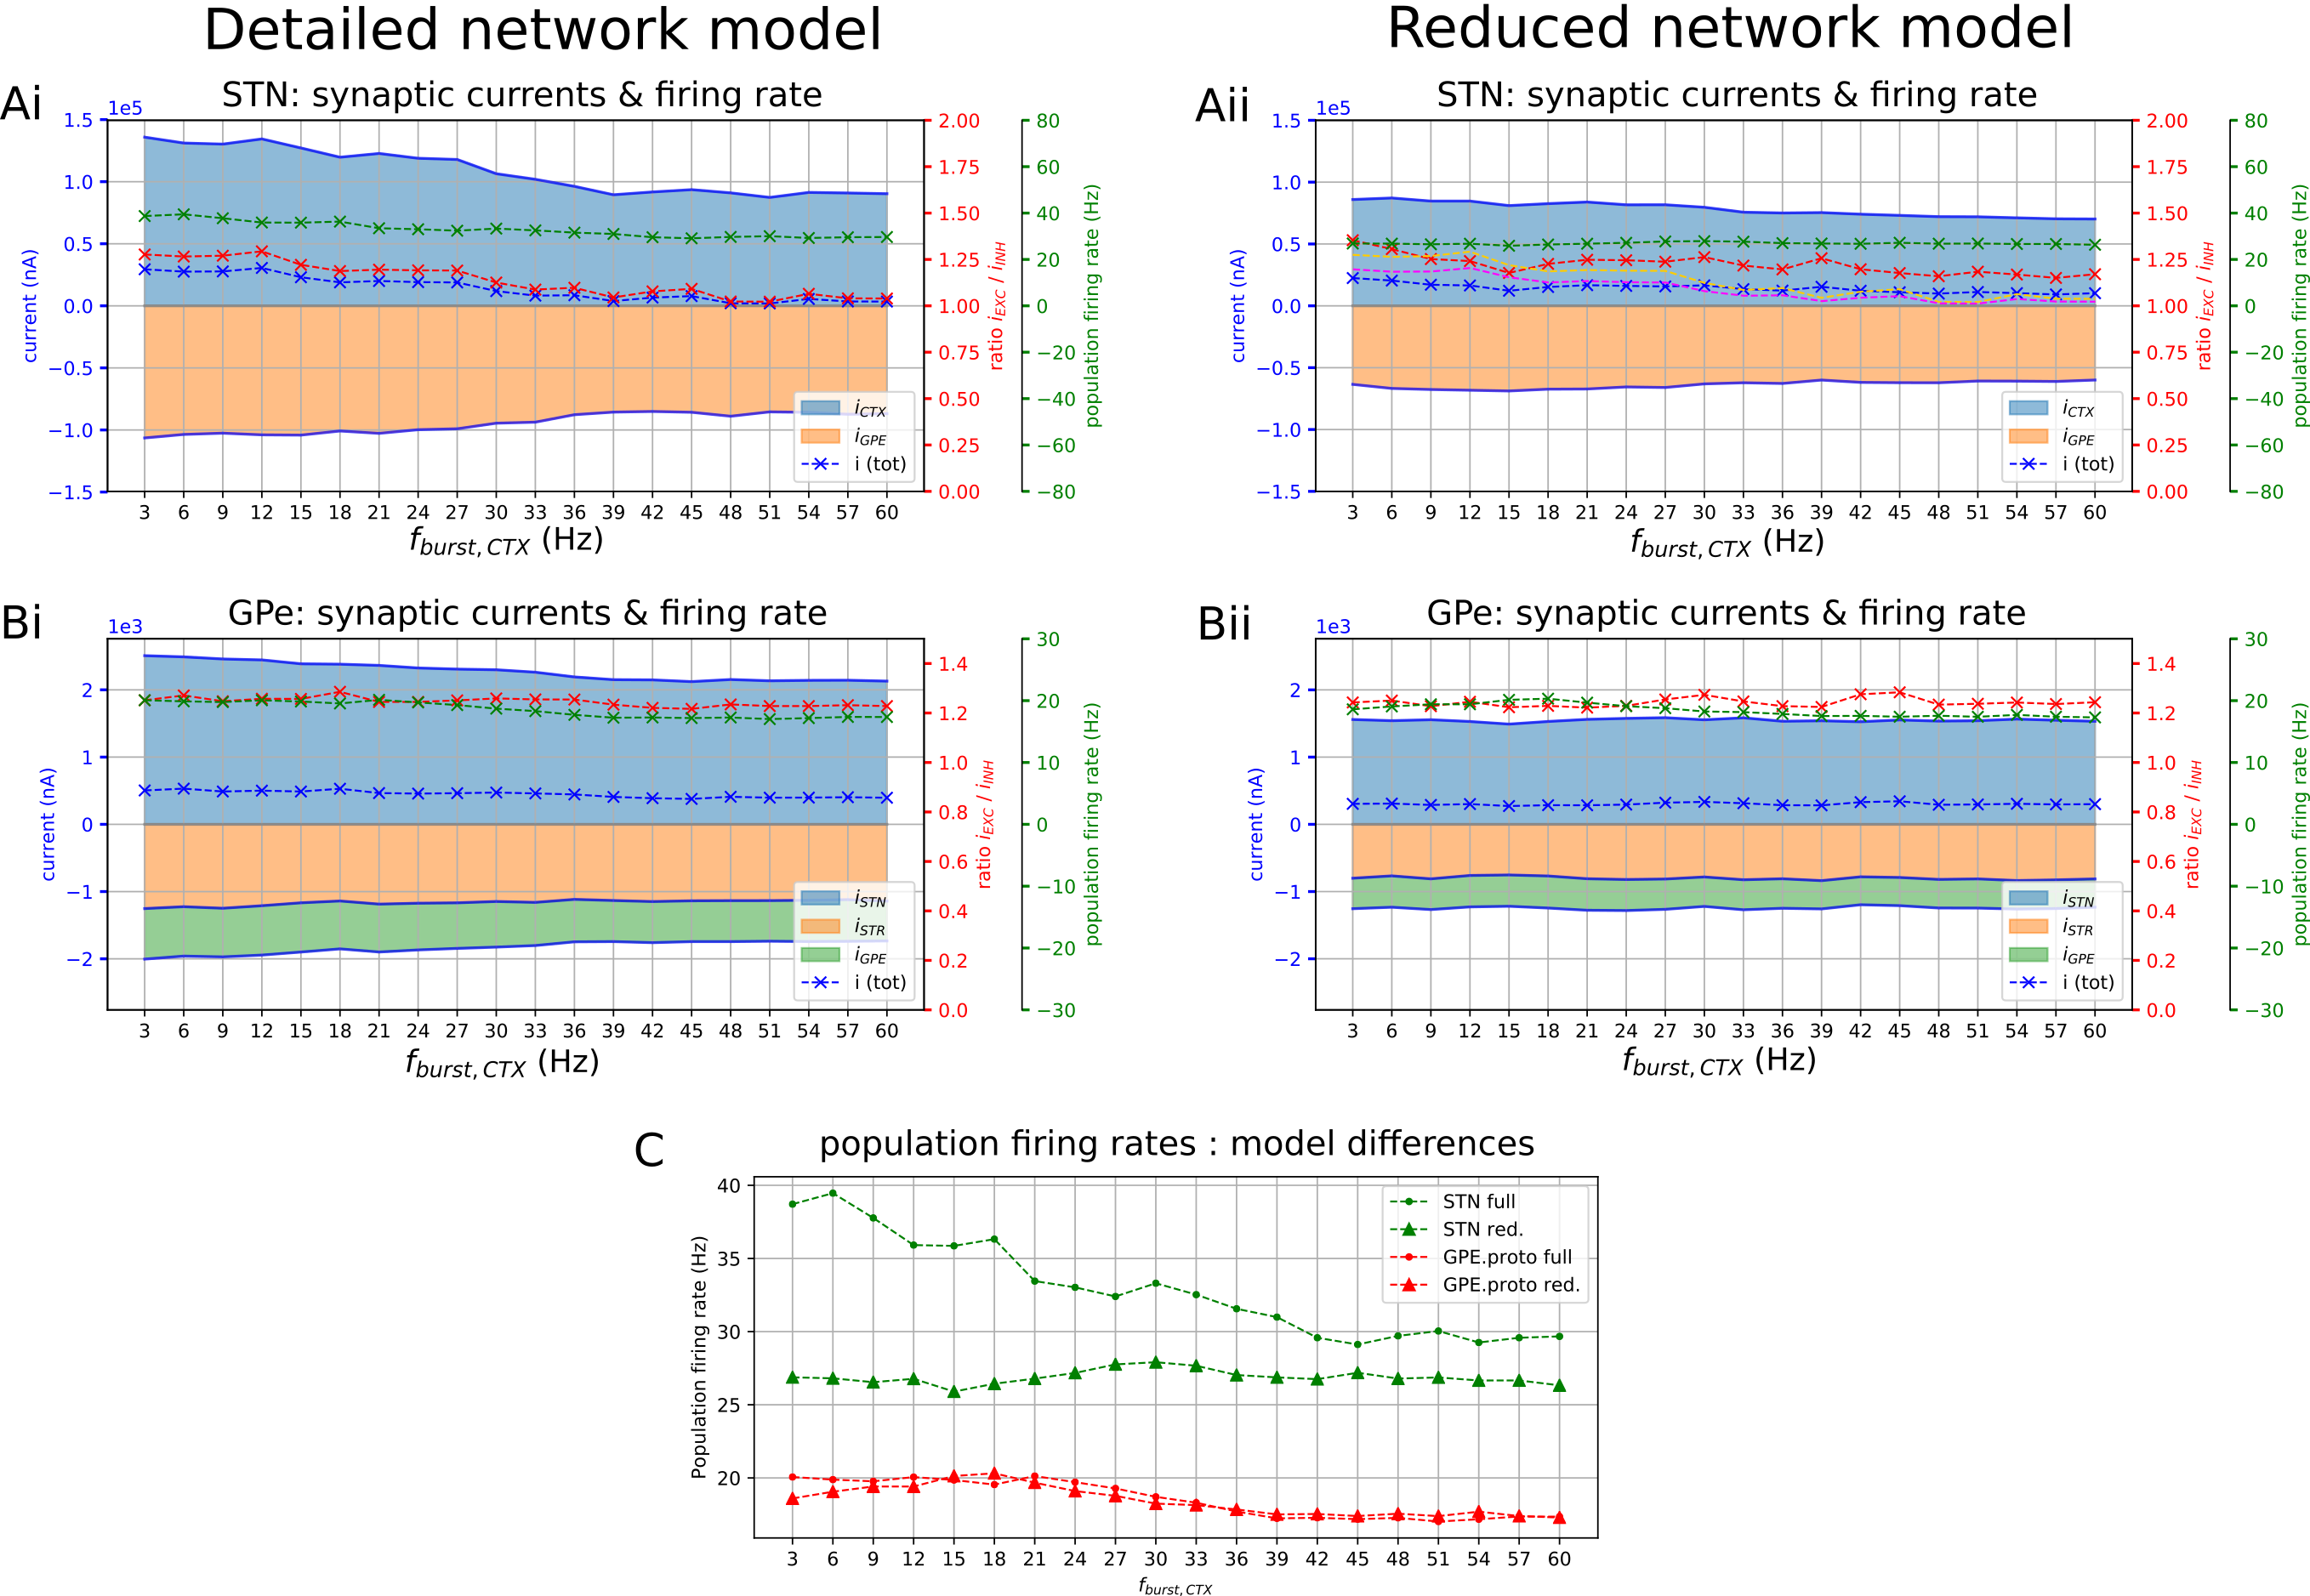
\includegraphics[width=\textwidth]{ch_reduced_model/figs/fig_net-full-vs-red_sweep-f-burst-ctx_currents-EI.png}
\caption{
\textbf{Total synaptic current delivered to STN and GPe neurons and its effect on firing rates.}
\textbf{A-B}: Balance of excitation and inhibition in the STN (A) and GPe (B) based on synaptic currents recorded in three neurons. Results for detailed model in column i (left) and reduced model in column ii (right).
Population firing rate (green), E/I ratio (red), and net synaptic current (blue). Shaded areas represent estimated total synaptic current from one pre-synaptic population during a simulation. Total synaptic current delivered
is lower for both excitatory and inhibitory synapses in STN and GPe. The balance of excitation and inhibition
and population firing rate are not strongly affected in the GPe model but they are in the STN model.
\textbf{C}: Differences in population firing rates for increasing cortical oscillation frequency, in detailed model (dots), and reduced model (triangles).
}
\label{fig:net-full-vs-red_sweep-f-burst_currents-EI}
\end{figure}

%
%

A third key behavior of the detailed network model was that the strength of
beta-band resonance in the STN-GPe feedback loop could be varied by increasing
the level of cortical excitation (see Chapter~\ref{ch3:detailed-model}, Fig.~\ref{fig:exogenous_ctx-resonance-example_A-psd-currents}).
%
The reduced network model also exhibited this behavior but the point where
maximal 20 Hz resonance occurred was at a higher value of CTX-STN synapse strength
(Fig.~\ref{fig:net-full-vs-red_ctx-burst_sweep-g-ctx-stn}).
The shift of the resonance peak was related to features of the spiking patterns of STN neurons:
comparing spike features at a synaptic scale factor of 0.7 (Fig.~\ref{fig:net-full-vs-red_ctx-burst_sweep-g-ctx-stn}.C, D),
STN spiking is sparser in the reduced model (17.7 Hz, 23.0 Hz in reduced/detailed model,
respectively), the mean intra-burst firing rate is higher (101 Hz vs 87 Hz)
and bursts appear shorter without a prominent tail with reduced firing rate
(Fig.~\ref{fig:net-full-vs-red_ctx-burst_sweep-g-ctx-stn}.C).
%

%
%
%
%
%

\begin{figure}[ht]
\centering
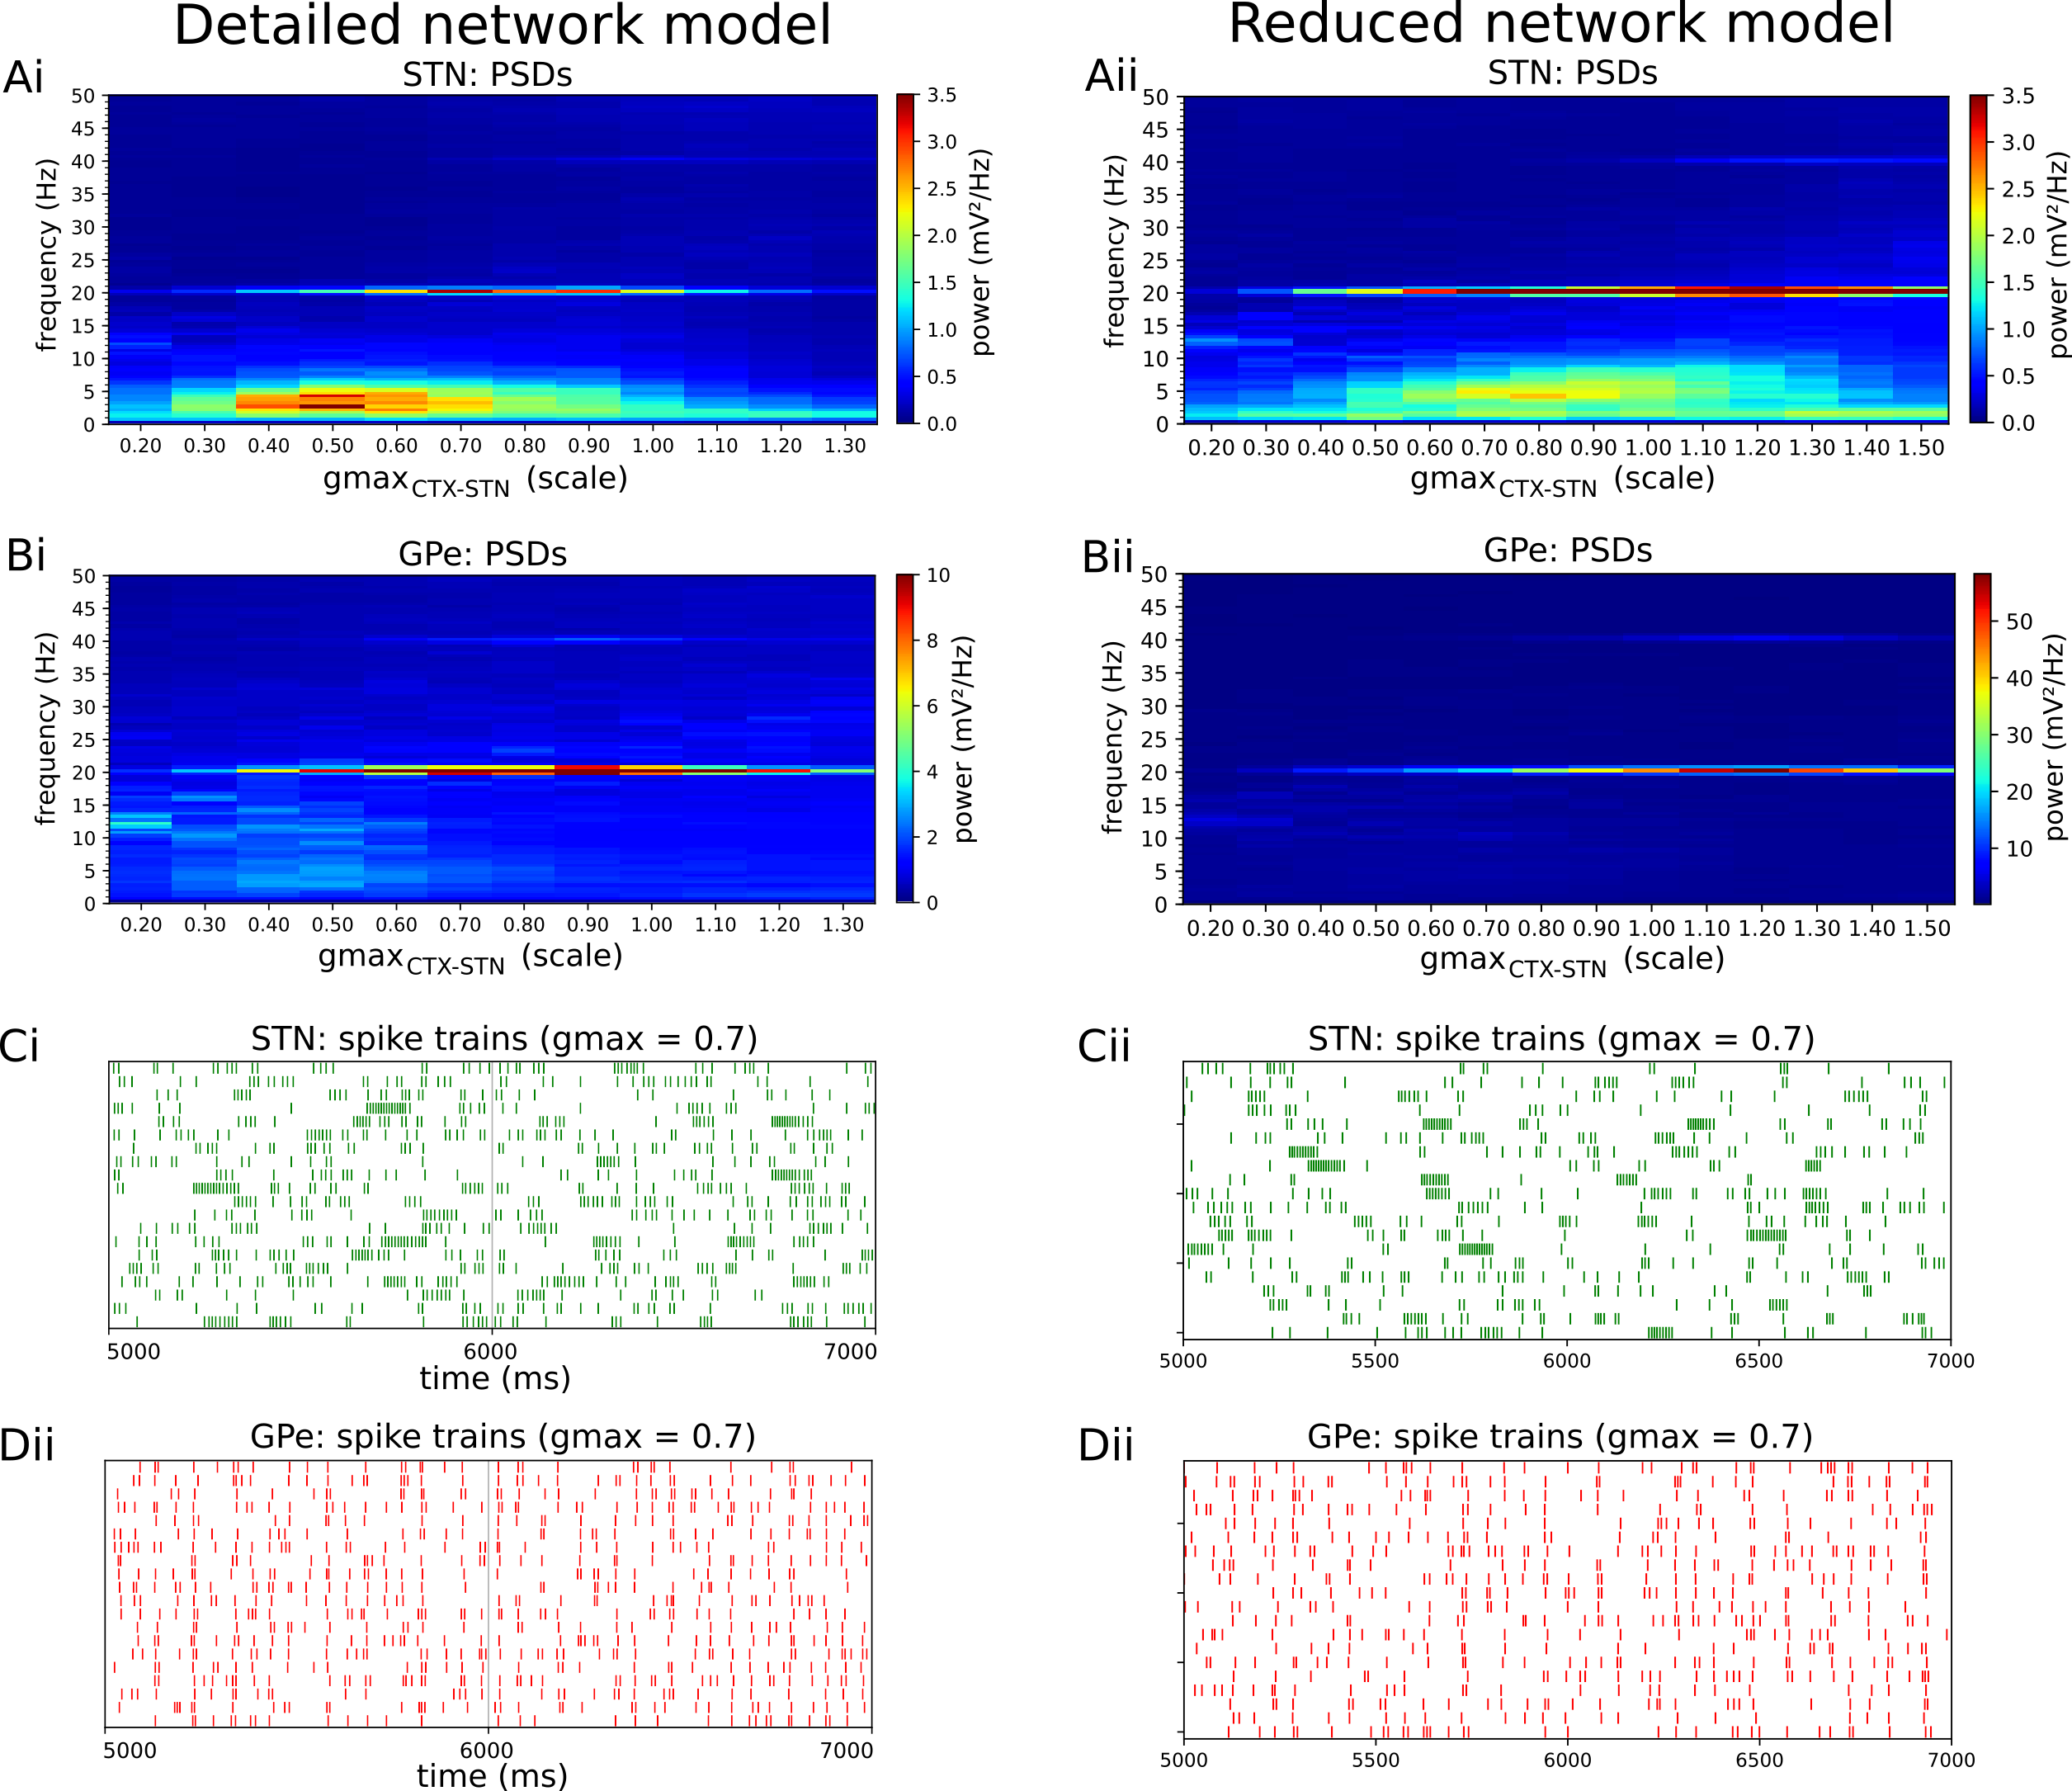
\includegraphics[width=\textwidth]{ch_reduced_model/figs/fig_net-full-vs-red_sweep-g-ctx-stn_f-burst-20.png}
\caption{
\textbf{Cortico-subthalamic excitation level determines strength of beta-band resonance in the STN-GPe loop.}
Power spectral densities and spike raster plots for the detailed network model (column i, left) and network using reduced neuron models (column ii, right). Mean power spectral density (PSD) of somatic membrane voltages of STN neurons \textbf{(A)} and GPe neurons \textbf{(B)}. Note different color scales in \textbf{(B)}. Representative spike trains for STN \textbf{(C)} and GPe population \textbf{(D)} for intermediate level of cortical excitation corresponding to low-frequency bursting regimen. Varying the strength of CTX-STN synapses changes the strength of 20 Hz resonance but maximum resonance occurs at different points in the detailed and reduced network models.
}
\label{fig:net-full-vs-red_ctx-burst_sweep-g-ctx-stn}
\end{figure}

%
%
%
\section{Discussion}
%
%
%
%
%
%
%
%
%
%
%
%
%
%

%
%
%
%
%
%

%
%
%
%
%
%


%
A reduced model of the STN-GPe network that retains key properties of a biophysically
detailed model is presented. The model was generated in an automated fashion based
on cellular morphology reduction algorithms applied to the multi-compartment cell
models that make up the detailed network model. The reduced network model represents
a reduction in state variables of 85.5 \% and computation time of 79 \% over the
detailed model. This study demonstrates that reduced models of neuronal networks
can be constructed with relative ease based on detailed characterizations of the component cells.
The reduced network model retains the same phenomenological behavior with
only small differences in quantitative properties such as mean population firing rates.
Such reduced models are computationally more efficient and may be more appropriate
to explore the network behavior under different input and parameter settings when
the use of more complex models is not feasible. Furthermore, they offer the prospect
of fast implementations of network models that can enable real-time
optimization of stimulation parameters in the clinic.

%
\subsection{Neuronal morphology reduction}
%
%
%

The algorithm for the reduction of detailed neuronal morphologies into equivalent cable
structures used here followed the approach of conserving the axial resistance per
unit length but not the surface area, first described in~\cite{bush_reduced_1993}.
This algorithm was extended in \cite{marasco_fast_2012} using empirical scaling
rules to handle the case of dendritic active and synaptic conductances.
This approach was chosen because active dendritic conductances were present
in the STN and GPe neuron models. However, the algorithm was modified
by altering the way compartments were clustered and merged into equivalent
cables. Rather than recursively merging cylindrical compartments as in
\cite{marasco_fast_2012}, yielding an equivalent cable with uniform diameter,
the clustering approach of \cite{douglas1992exploring} was followed, preserving
the gradual tapering of neurite diameters with distance from the soma.
It was found that this method yielded a better match in burst responses
mediated by dendritic ion channels in STN neurons. This was related to the
higher local input impedance in the distal dendrites obtained using this method.

\cite{hendrickson_capabilities_2011} and \cite{elbasiouny_development_2014}
previously investigated the capabilities of reduced morphology models to conserve the
response properties of detailed models. They concluded that responses that depend
strongly on  dendritic input impedance and activation of dendritic active channels are not
accurately reproduced by such models. However, they show that their accuracy can be improved by
limiting the level of reduction, maintaining a degree of branching in the equivalent cables.
%
%
%
The results support these conclusions: the choice of a reduction method resulting
in tapering equivalent cables as well as the conservation of dendritic branching
all served to obtain a better match in input impedance properties.
Specifically, it was found to be necessary to limit the reduction to the merging of sections
starting at each dendritic trunk section, resulting in a branched model rather than
a single equivalent cable (data not shown). Despite these choices, the bursting
response of STN neurons, which is mediated by dendritic active currents, was still
not fully preserved in the reduced cell model.

%
%
\subsubsection{GPe model}
An alternative morphology reduction algorithm was used in \cite{hendrickson_capabilities_2011}
to construct equivalent cable models of the same detailed GPe model used in
this study \cite{gunay_channel_2008}. The algorithm used in that study preserves the total
surface area of equivalent cables and outward passive attenuation of voltages,
yielding cables with larger diameters without monotonic outward tapering \cite{destexhe_simplified_2001,tobin_creation_2006}. This algorithm was not
used in this study because tapering diameters were found necessary to match responses
of the STN model. It is possible that this requirement is less important in the
GPe model because ion channel densities are distributed uniformly in that model,
and it has no characteristic responses mediated solely by distally distributed
ion channels.
%
Stereotypical responses of the GPe model were faithfully reproduced by the
reduced model presented here (Fig.~\ref{fig:gpe-full-vs-red_protos-clamp})
and phase response curves also showed an excellent match (Fig.~\ref{fig:gpe-full-vs-red_PRC-curves}).
Note that in the original \cite{gunay_channel_2008} GPe neuron model, the diameter and length of each
compartment were normalized to 1 micron in length. This limitation
was preserved since it was necessary to match the neuron's responses
to the published ones using the published parameter values.
As a result, the cell is spatially and electrically compact, reflected in
the relatively small variation in transfer and input impedances throughout the
dendritic structure (Fig.~\ref{fig:gpe-full-vs-red_Zin-Ztr}.A,B).
%
Responses of the detailed GPe neuron model published by \cite{gunay_channel_2008}
were also reproduced by the reduced model of \cite{hendrickson_capabilities_2011}.
Moreover, a single-compartment version of this model was derived in \cite{fujita_influences_2012}
and infinitesimal PRC, a different type of PRC valid under the assumptions of weakly coupled oscillator
theory, are derived. This single-compartment model also reproduced the stereotypical
responses tested here.
%

%
%
\subsubsection{STN model}
The reduced STN neuron model showed small differences in its responses compared
to the detailed model (Fig.~\ref{fig:stn-full-vs-red_protos-clamp}). Burst and
plateau responses were shortened in duration leading to a smaller number
of spikes per burst. This shortening was related to the dynamics of generation
and termination of the $Ca^{2+}$-mediated plateau originating in the distal
regions of the dendrites. These dynamics are regulated by the interplay of
voltage-gated CaT, CaL, and sKCa channels with local membrane voltage dynamics
\cite{gillies_membrane_2005}. In the reduced model, the reduced input impedance
in distal dendrites results in lower-amplitude membrane voltage depolarizations,
leading to altered dynamics of voltage-dependent channel gating variables.
Specifically, due to decreased gate open fractions, the amplitude of
ionic currents is lowered (data not shown), resulting in shortening
of the self-sustaining CaT-mediated plateau.
%
%
Phase response curves matched well with those of the detailed model when fitted curves were
compared. However, there was a large variability in phase shifts
in some regions of the PRC. Particularly for inhibitory stimuli arriving
at late phases, and distal excitatory phases arriving at early phases
the variability was high (Fig.~\ref{fig:stn-full-vs-red_PRC-curves}.B, C).
This variability is related to the randomization of stimulus timings
during measurement of the PRC: because stimulus timings are randomized
in successive ISIs, their residual influence in the following ISI
varies between PRC samples. This residual influence is determined both
by passive dissipation of stimulus-induced PSP and the interaction
with ion channel currents through voltage-gated states. Because several
gating variables have long time constants, the residual influence of
the associated ionic currents is considerable in some sampled ISIs.
%
%
%
%
%
%
%
Hence, while the phase response characteristic of STN neurons
is preserved by the morphology reduction method, the altered electrical properties
resulting from the collapsing of neurites limit its ability to faithfully
reproduce responses in the reduced model.


%
%
%
%
%
%
%
Synaptic phase response curves of rat STN neurons were measured experimentally
by \cite{farries_phase_2012}. In that study, excitatory PRC were pure type I,
causing only phase advancement, unlike in the current model. There are multiple factors
that could explain the discrepancy of the measured PRC. The negative part of the
PRC that occurs for phases $>$ 1 in the current study occurs because the definition of
$\Delta \phi$, which is measured with respect to the mean ISI (equation \ref{eq:prc-samples}).
Moreover, samples occurring at phases slightly smaller than 1 in this study can have an associated
PSP occurring at $t > T_{mean}$, resulting in a $\Delta \phi$ that is also by definition negative.
This is because stimulus times are defined here as the time of spike arrival at the synapse,
whereas in \cite{farries_phase_2012} the stimulus time was taken to be the time halfway through the PSP.
However, the negative part of STN PRC occurring at $0.8 < \phi < 1.0 $ is clearly different
from the study by \cite{farries_phase_2012} and is not accounted for by differences in
the calculation method. This could result from the fact that PRC were measured in this study
while STN neurons were in a more excited state (made to fire at 20 Hz), whereas in
the study by \cite{farries_phase_2012} they were measured during slower spontaneous firing.
Moreover, the magnitude of post-synaptic potentials are different.
The different membrane polarization level as a result of these factors could cause interactions
with voltage-gated channels that do not occur during spontaneous firing.
Alternatively, there could be differences in the membrane dynamics captured by the
\cite{gillies_membrane_2005} STN neuron model and present in the biological neurons
recorded by \cite{farries_phase_2012}.

A single compartment model of the STN projection neuron by \cite{otsuka_conductance-based_2004}
also has the capability to generate plateau potentials and rebound bursts,
and an earlier single-compartment model by \cite{terman_activity_2002} likewise
exhibits the rebound burst response. These cell models were not used in the network
model presented here because of the lack of a branching dendritic structure, resulting
in different processing properties of synaptic inputs, as shown in other neuron types \cite{hendrickson_capabilities_2011,elbasiouny_development_2014}.
In particular, the propensity of single-compartment models to burst when embedded
in network models was found to be lower compared to branch models, based on
other simulation experiments (data not shown). This is likely related to
the ability of different dendritic regions to act as semi-independent subunits
that are electrically separated in multi-compartment models \cite{wybo_electrical_2019}.
However, to establish this quantitatively, detailed comparisons of the
responses to synaptic inputs between single-compartment and multi-compartment
neuron models with various degrees of reduction should be performed.

%
\subsection{Network model}

%
Key oscillatory and synchronization properties of the detailed STN-GPe network
model were conserved in the reduced model (Fig.~\ref{fig:net-full-vs-red_spont_sweep-g-ctx-stn} -
\ref{fig:net-full-vs-red_ctx-burst_sweep-g-ctx-stn}).
%
Endogenously generated oscillations in the network (Fig.~\ref{fig:net-full-vs-red_spont_sweep-g-ctx-stn}),
resonance with cortical oscillatory bursting activity (Fig.~\ref{fig:net-full-vs-red_sweep-f-burst}),
and modulation of resonance strength by the level of excitation (Fig.~\ref{fig:net-full-vs-red_ctx-burst_sweep-g-ctx-stn}) were exhibited by both models.
%
However, the changes in electrical properties of the cell models introduced changes
in the integration of synaptic currents and their interaction with intrinsic ionic currents
through the local membrane voltage. The total synaptic current delivered during
network simulation was smaller in the reduced cell models (Fig.~\ref{fig:net-full-vs-red_sweep-f-burst_currents-EI}).
In STN neurons this was accompanied by a shift in the balance of currents toward
slightly higher excitation and, paradoxically, a lower firing rate.
The decrease in synaptic current delivered is likely related to the mutual shunting of
synapses \cite{segev_what_2006} lumped closer together in the dendritic trees
of the reduced models compared to the detailed morphologies, were they were more
spatially and electrically distant due to the higher degree of branching (Fig.
\ref{fig:stn-full-vs-red_Zin-Ztr}, \ref{fig:gpe-full-vs-red_Zin-Ztr}).
Furthermore, the reduction in firing rate could be due to the increased effectiveness of
perisomatic inhibition in the more compact reduced neuron model.
%

%
The downward frequency shift of the resonance peak in the reduced network model
(Fig.~\ref{fig:net-full-vs-red_sweep-f-burst}), and the higher level of excitatory
drive required to reach peak 20-Hz resonance (Fig.~\ref{fig:net-full-vs-red_spont_sweep-g-ctx-stn})
mirror the results of Chapter~\ref{ch3:detailed-model}: since the firing rates are
lower in the reduced model at equal synaptic strengths, the discrepancy between
Fig.~\ref{fig:net-full-vs-red_ctx-burst_sweep-g-ctx-stn}.A and B can be partly explained by noting that
region of E/I values sampled wile increasing the synaptic conductance is moved to the left on the curves of
Fig.~\ref{fig:exogenous_ctx-resonance-response_B-vectorlength}.
%
However, this does not explain the stronger beta-band power in the reduced network model
compared to the detailed model (Fig.~\ref{fig:net-full-vs-red_ctx-burst_sweep-g-ctx-stn}.Aii - Bii).
Because power spectra were computed from somatic membrane voltages in each population,
spectral power at 20 Hz is related to the sinusoidal character of the STN neuron's membrane voltages:
the shorter bursts with increased intra-burst firing rate and sparser firing between bursts
in the reduced model ((Fig.~\ref{fig:net-full-vs-red_ctx-burst_sweep-g-ctx-stn}.Ci - Cii))
contribute to sharpening of the sinusoidal profile.

%
%
%

%
\subsection{Limitations and future work}
%
%
%
%
%

%
%
%
%
%
%
%

%
When reducing a detailed morphology to an equivalent cable model, the properties of
the resulting model depend strongly on the reduction algorithm used, the trade-offs
inherent in the algorithm, and the choice of its parameters such as the degree of reduction.
Further studies are needed to show which reduction algorithms and parameter choices
are the most suitable to reproduce specific aspects of neuron and neuronal network behavior.
Furthermore, the optimal method might also depend on the specific complement of ion channels present in
the cell and its spatial distribution in the dendritic tree. An additional concern
when choosing a reduction method is the size of the network and its connectivity,
which determine the number of synapses modeled on each cell. As this number increases,
more synapses are lumped together in the same or neighboring compartments, warranting
different degrees of reduction to avoid excessive mutual shunting effects. Firing rates
and patterns should also be taken into account, as they determine the degree of temporal
overlap of post-synaptic potentials.

%
Another open question is the use of reduced morphology models to study the effects
of extracellular electrical stimulation. Given that all morphology reduction algorithms
alter aspects of the electrical cable representation of the cell, reproducing the effect
of a distributed time-varying voltage source might prove challenging.
Moreover, like synapses, extracellular stimulation
activates ion channels through local membrane voltage fluctuations \cite{johnson_quantifying_2008}
that are dependent on the cell's electrotonic properties such as local input impedance.
Hence, reproducing the effects of electrical stimulation is another goal that warrants
careful selection of reduction algorithms and characterization of its effects.


%
%
An alternative approach to bottom-up reduction of neuron models is state space reduction
of membrane dynamics, as in \cite{fitzhugh_impulses_1961} and \cite{morris_voltage_1981}.
In this approach, the number of state variables describing the membrane dynamics in each
neuronal compartment is reduced by analyzing their trajectories in phase space %
and projecting them to a lower dimensional space. This reduction approach has only been
applied to single compartment neuron models so far. Extending it to multi-compartmental
neuron models could potentially preserve the influence of neuron geometries on their
responses to electrical stimulation. However, the reduction of voltage-dependent dynamics
of individual ion channel states to lower-dimensional trajectories would then also
have to account for the effect of extracellular time-varying voltage sources.
%
%
%
Another approach that foregoes coupling the electrical model to the neural network model
during the simulation is to use the insights about cellular activation from a detailed model
(as in Chapter~\ref{ch4:dbs-model}) to make assumptions about which cellular structures are activated.
%
Eliminating the requirement for coupling the electrical model to the neuronal cable models
can substantially reduce the computation time.


%
Phase response curves have been used to predict the synchronization properties
of neuronal networks based on network topology and connection types
\cite{achuthan_phase-resetting_2009,netoff_synchronization_2005,acker_synchronization_2003}.
In the current study however, they were used after the morphology reduction process, %
in combination with voltage responses, to assess the quality of the reduction
before the network behavior was simulated. Moreover, PRC were not used
as part of a parameter selection scheme or optimization routine to determine
the reduction parameters.
To serve as a predictor of the quality of a model reduction algorithm or parameter set, %
PRC of cells reduced using different algorithms and different degrees of reduction
would need to compared, together with the resulting network behavior.
The error between PRCs and predicted synchronization properties can then be quantified
using appropriate distance functions. In future studies, PRC could
then be integrated in the cost function of an optimization routine to search the
parameter space of the reduction algorithm for the optimal degree of reduction
and clustering scheme for dendritic regions.

%
%
%
%
The results suggest a reduction in computation time that is proportionate to the reduction
in the number of state variables. However, the effects of computational resource
allocation and load balance between computing nodes during parallel simulations was not systematically
explored. Substantial speed-ups may be obtained when the load balance is optimized
for each model \cite{migliore_parallel_2006}. Hence it is possible that in the best-case
scenario for load balance in each model, the speed-up achievable is larger than
observed here.
%
%
%
%
%
%
However, if in the best-case scenario, the reduction in computation time is
proportional to the number of state variables, and if dendritic branching
must be retained to preserve cellular responses and synaptic integration properties,
as suggested by \cite{hendrickson_capabilities_2011,elbasiouny_development_2014} for
different neuron models, the improvements in computation time can not be expected to
exceed one order of magnitude. Taking these numbers into account, it is suggested
that the advantages and limitations are carefully considered before opting to
use morphology  reduction methods.
%


%
\subsection{Conclusion}
%

In summary, a bottom-up model reduction method for network models based
on the substitution of equivalent cable models for morphologically detailed
cell model is presented. The method was used to reduce a biophysically
detailed model of the STN-GPe network to an equivalent network model with
a reduced number of state variables and lower computational complexity.
While key properties of the original network model were
preserved, firing patterns and the response to synchronous inputs were
subtly altered: burst responses were shortened, influencing power spectra
of neuronal activation patterns, and there was a frequency shift in the
resonance peak shown in the frequency response of the original model.
%
%
These differences in firing patterns can be related back to the inability of
the morphology reduction method to precisely preserve neuronal responses that
are strongly dependent on dendritic ion channel engagement, which is most
evident in the burst responses generated by STN neurons.
%
Moreover, these results shows that small differences in individual cell properties
pre- and post-reduction can lead to differences in emergent activity patterns.
The observed differences in the spiking patterns and frequency response
of the network were quantitatively small however, and may be improved in the future by
adding compensatory changes in synaptic scaling or electrical cell parameters
that need to be further investigated. These results indicate that neuronal
morphology reduction methods can be a valuable approach to study the responses
of large networks of cells that maintain a close relationship to the underlying
physiology. Due to their reduced computational complexity, the resulting
network models could be used for the design and testing of DBS protocols in
silico, when subcellular biophysical interactions need to be accounted for.

